% Options for packages loaded elsewhere
\PassOptionsToPackage{unicode}{hyperref}
\PassOptionsToPackage{hyphens}{url}
%
\documentclass[
]{book}
\usepackage{lmodern}
\usepackage{amssymb,amsmath}
\usepackage{ifxetex,ifluatex}
\ifnum 0\ifxetex 1\fi\ifluatex 1\fi=0 % if pdftex
  \usepackage[T1]{fontenc}
  \usepackage[utf8]{inputenc}
  \usepackage{textcomp} % provide euro and other symbols
\else % if luatex or xetex
  \usepackage{unicode-math}
  \defaultfontfeatures{Scale=MatchLowercase}
  \defaultfontfeatures[\rmfamily]{Ligatures=TeX,Scale=1}
\fi
% Use upquote if available, for straight quotes in verbatim environments
\IfFileExists{upquote.sty}{\usepackage{upquote}}{}
\IfFileExists{microtype.sty}{% use microtype if available
  \usepackage[]{microtype}
  \UseMicrotypeSet[protrusion]{basicmath} % disable protrusion for tt fonts
}{}
\makeatletter
\@ifundefined{KOMAClassName}{% if non-KOMA class
  \IfFileExists{parskip.sty}{%
    \usepackage{parskip}
  }{% else
    \setlength{\parindent}{0pt}
    \setlength{\parskip}{6pt plus 2pt minus 1pt}}
}{% if KOMA class
  \KOMAoptions{parskip=half}}
\makeatother
\usepackage{xcolor}
\IfFileExists{xurl.sty}{\usepackage{xurl}}{} % add URL line breaks if available
\IfFileExists{bookmark.sty}{\usepackage{bookmark}}{\usepackage{hyperref}}
\hypersetup{
  pdftitle={R4DS Exercise Solutions},
  pdfauthor={Maddie},
  hidelinks,
  pdfcreator={LaTeX via pandoc}}
\urlstyle{same} % disable monospaced font for URLs
\usepackage{color}
\usepackage{fancyvrb}
\newcommand{\VerbBar}{|}
\newcommand{\VERB}{\Verb[commandchars=\\\{\}]}
\DefineVerbatimEnvironment{Highlighting}{Verbatim}{commandchars=\\\{\}}
% Add ',fontsize=\small' for more characters per line
\usepackage{framed}
\definecolor{shadecolor}{RGB}{248,248,248}
\newenvironment{Shaded}{\begin{snugshade}}{\end{snugshade}}
\newcommand{\AlertTok}[1]{\textcolor[rgb]{0.94,0.16,0.16}{#1}}
\newcommand{\AnnotationTok}[1]{\textcolor[rgb]{0.56,0.35,0.01}{\textbf{\textit{#1}}}}
\newcommand{\AttributeTok}[1]{\textcolor[rgb]{0.77,0.63,0.00}{#1}}
\newcommand{\BaseNTok}[1]{\textcolor[rgb]{0.00,0.00,0.81}{#1}}
\newcommand{\BuiltInTok}[1]{#1}
\newcommand{\CharTok}[1]{\textcolor[rgb]{0.31,0.60,0.02}{#1}}
\newcommand{\CommentTok}[1]{\textcolor[rgb]{0.56,0.35,0.01}{\textit{#1}}}
\newcommand{\CommentVarTok}[1]{\textcolor[rgb]{0.56,0.35,0.01}{\textbf{\textit{#1}}}}
\newcommand{\ConstantTok}[1]{\textcolor[rgb]{0.00,0.00,0.00}{#1}}
\newcommand{\ControlFlowTok}[1]{\textcolor[rgb]{0.13,0.29,0.53}{\textbf{#1}}}
\newcommand{\DataTypeTok}[1]{\textcolor[rgb]{0.13,0.29,0.53}{#1}}
\newcommand{\DecValTok}[1]{\textcolor[rgb]{0.00,0.00,0.81}{#1}}
\newcommand{\DocumentationTok}[1]{\textcolor[rgb]{0.56,0.35,0.01}{\textbf{\textit{#1}}}}
\newcommand{\ErrorTok}[1]{\textcolor[rgb]{0.64,0.00,0.00}{\textbf{#1}}}
\newcommand{\ExtensionTok}[1]{#1}
\newcommand{\FloatTok}[1]{\textcolor[rgb]{0.00,0.00,0.81}{#1}}
\newcommand{\FunctionTok}[1]{\textcolor[rgb]{0.00,0.00,0.00}{#1}}
\newcommand{\ImportTok}[1]{#1}
\newcommand{\InformationTok}[1]{\textcolor[rgb]{0.56,0.35,0.01}{\textbf{\textit{#1}}}}
\newcommand{\KeywordTok}[1]{\textcolor[rgb]{0.13,0.29,0.53}{\textbf{#1}}}
\newcommand{\NormalTok}[1]{#1}
\newcommand{\OperatorTok}[1]{\textcolor[rgb]{0.81,0.36,0.00}{\textbf{#1}}}
\newcommand{\OtherTok}[1]{\textcolor[rgb]{0.56,0.35,0.01}{#1}}
\newcommand{\PreprocessorTok}[1]{\textcolor[rgb]{0.56,0.35,0.01}{\textit{#1}}}
\newcommand{\RegionMarkerTok}[1]{#1}
\newcommand{\SpecialCharTok}[1]{\textcolor[rgb]{0.00,0.00,0.00}{#1}}
\newcommand{\SpecialStringTok}[1]{\textcolor[rgb]{0.31,0.60,0.02}{#1}}
\newcommand{\StringTok}[1]{\textcolor[rgb]{0.31,0.60,0.02}{#1}}
\newcommand{\VariableTok}[1]{\textcolor[rgb]{0.00,0.00,0.00}{#1}}
\newcommand{\VerbatimStringTok}[1]{\textcolor[rgb]{0.31,0.60,0.02}{#1}}
\newcommand{\WarningTok}[1]{\textcolor[rgb]{0.56,0.35,0.01}{\textbf{\textit{#1}}}}
\usepackage{longtable,booktabs}
% Correct order of tables after \paragraph or \subparagraph
\usepackage{etoolbox}
\makeatletter
\patchcmd\longtable{\par}{\if@noskipsec\mbox{}\fi\par}{}{}
\makeatother
% Allow footnotes in longtable head/foot
\IfFileExists{footnotehyper.sty}{\usepackage{footnotehyper}}{\usepackage{footnote}}
\makesavenoteenv{longtable}
\usepackage{graphicx,grffile}
\makeatletter
\def\maxwidth{\ifdim\Gin@nat@width>\linewidth\linewidth\else\Gin@nat@width\fi}
\def\maxheight{\ifdim\Gin@nat@height>\textheight\textheight\else\Gin@nat@height\fi}
\makeatother
% Scale images if necessary, so that they will not overflow the page
% margins by default, and it is still possible to overwrite the defaults
% using explicit options in \includegraphics[width, height, ...]{}
\setkeys{Gin}{width=\maxwidth,height=\maxheight,keepaspectratio}
% Set default figure placement to htbp
\makeatletter
\def\fps@figure{htbp}
\makeatother
\setlength{\emergencystretch}{3em} % prevent overfull lines
\providecommand{\tightlist}{%
  \setlength{\itemsep}{0pt}\setlength{\parskip}{0pt}}
\setcounter{secnumdepth}{5}
\usepackage{booktabs}
\usepackage{amsthm}
\makeatletter
\def\thm@space@setup{%
  \thm@preskip=8pt plus 2pt minus 4pt
  \thm@postskip=\thm@preskip
}
\makeatother
\usepackage[]{natbib}
\bibliographystyle{apalike}

\title{R4DS Exercise Solutions}
\author{Maddie}
\date{2022-01-26}

\begin{document}
\maketitle

{
\setcounter{tocdepth}{1}
\tableofcontents
}
\hypertarget{chapter-3}{%
\chapter{Chapter 3}\label{chapter-3}}

\hypertarget{chapter-3.2.4-exercises}{%
\section{Chapter 3.2.4 Exercises}\label{chapter-3.2.4-exercises}}

\hypertarget{question-1-run-ggplotdata-mpg.-what-do-you-see}{%
\subsection{Question 1: Run ggplot(data = mpg). What do you see?}\label{question-1-run-ggplotdata-mpg.-what-do-you-see}}

\begin{Shaded}
\begin{Highlighting}[]
\KeywordTok{ggplot}\NormalTok{(}\DataTypeTok{data =}\NormalTok{ mpg) }
\end{Highlighting}
\end{Shaded}


\includegraphics{r4dsexercises_files/figure-latex/3.2.4 Question 1-1.pdf}

This line of code does not output a graph as there is no geom function to tell R studio what to output. Need `+ geom\_point(mapping = aes(x = displ, y = 'variable'))' to see anything

\hypertarget{question-2-how-many-rows-are-in-mpg-how-many-columns}{%
\subsection{Question 2: How many rows are in mpg? How many columns?}\label{question-2-how-many-rows-are-in-mpg-how-many-columns}}

234 rows, 11 columns

\hypertarget{question-3-what-does-the-drv-variable-describe-read-the-help-for-mpg-to-find-out.}{%
\subsection{Question 3: What does the drv variable describe? Read the help for ?mpg to find out.}\label{question-3-what-does-the-drv-variable-describe-read-the-help-for-mpg-to-find-out.}}

drv = the type of drive train, f = fwd, r = rwd, 4 = 4wd

\hypertarget{question-4-make-a-scatterplot-of-hwy-vs-cyl.}{%
\subsection{Question 4: Make a scatterplot of hwy vs cyl.}\label{question-4-make-a-scatterplot-of-hwy-vs-cyl.}}

\begin{Shaded}
\begin{Highlighting}[]
\KeywordTok{ggplot}\NormalTok{(}\DataTypeTok{data =}\NormalTok{ mpg) }\OperatorTok{+}
\StringTok{  }\KeywordTok{geom_point}\NormalTok{(}\DataTypeTok{mapping =} \KeywordTok{aes}\NormalTok{(}\DataTypeTok{x =}\NormalTok{ hwy, }\DataTypeTok{y =}\NormalTok{ cyl))}
\end{Highlighting}
\end{Shaded}

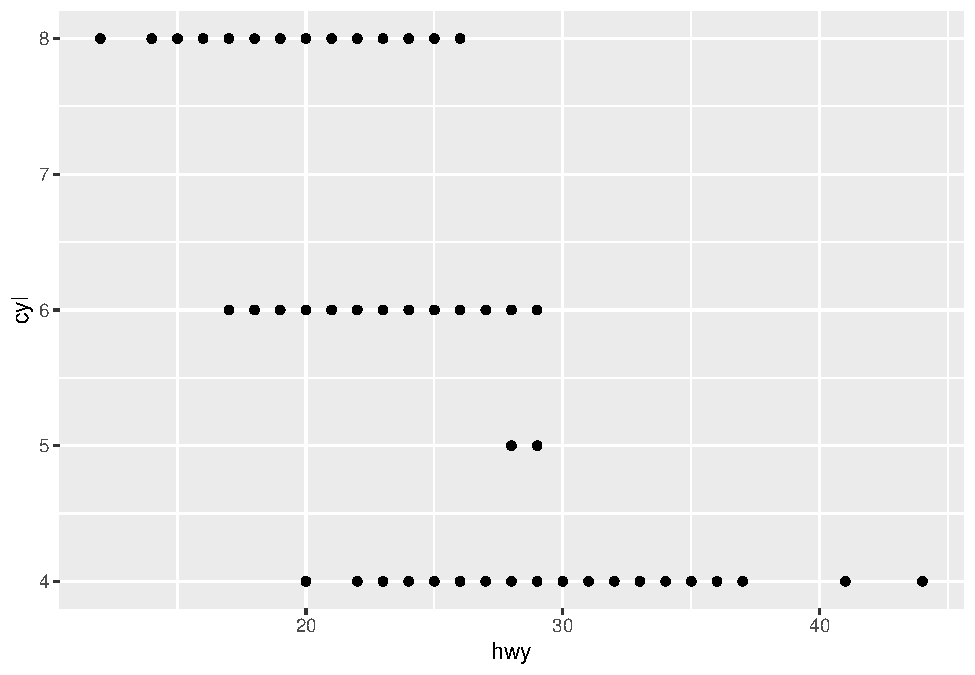
\includegraphics{r4dsexercises_files/figure-latex/3.2.4 Question 4-1.pdf}

\hypertarget{question-5-what-happens-if-you-make-a-scatterplot-of-class-vs-drv-why-is-the-plot-not-useful}{%
\subsection{Question 5: What happens if you make a scatterplot of class vs drv? Why is the plot not useful?}\label{question-5-what-happens-if-you-make-a-scatterplot-of-class-vs-drv-why-is-the-plot-not-useful}}

\begin{Shaded}
\begin{Highlighting}[]
\KeywordTok{ggplot}\NormalTok{(}\DataTypeTok{data =}\NormalTok{ mpg) }\OperatorTok{+}
\StringTok{  }\KeywordTok{geom_point}\NormalTok{(}\DataTypeTok{mapping =} \KeywordTok{aes}\NormalTok{(}\DataTypeTok{x =}\NormalTok{ class, }\DataTypeTok{y =}\NormalTok{ drv))}
\end{Highlighting}
\end{Shaded}

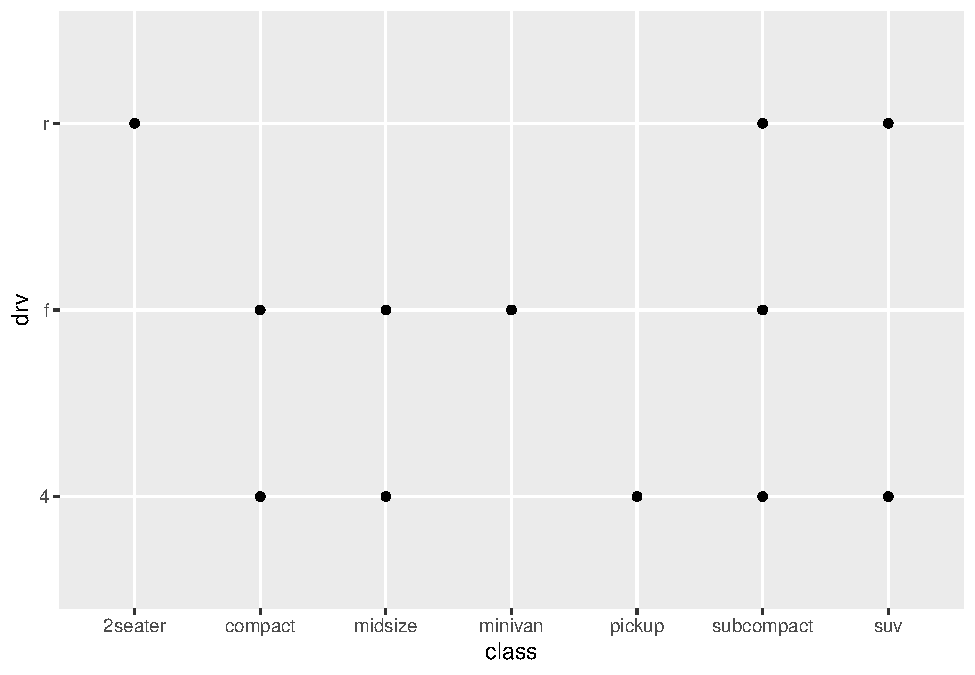
\includegraphics{r4dsexercises_files/figure-latex/3.2.4 Question 5-1.pdf}

This is not helpful because there are no numerical values in class or drv so a scatterplot wouldn't be a good way to visualize this data.

\hypertarget{chapter-3.3.1-exercises}{%
\section{Chapter 3.3.1 Exercises}\label{chapter-3.3.1-exercises}}

\hypertarget{question-1-whats-gone-wrong-with-this-code-why-are-the-points-not-blue}{%
\subsection{Question 1: What's gone wrong with this code? Why are the points not blue?}\label{question-1-whats-gone-wrong-with-this-code-why-are-the-points-not-blue}}

\begin{Shaded}
\begin{Highlighting}[]
\KeywordTok{ggplot}\NormalTok{(}\DataTypeTok{data =}\NormalTok{ mpg) }\OperatorTok{+}\StringTok{ }
\StringTok{  }\KeywordTok{geom_point}\NormalTok{(}\DataTypeTok{mapping =} \KeywordTok{aes}\NormalTok{(}\DataTypeTok{x =}\NormalTok{ displ, }\DataTypeTok{y =}\NormalTok{ hwy, }\DataTypeTok{color =} \StringTok{"blue"}\NormalTok{))}
\end{Highlighting}
\end{Shaded}

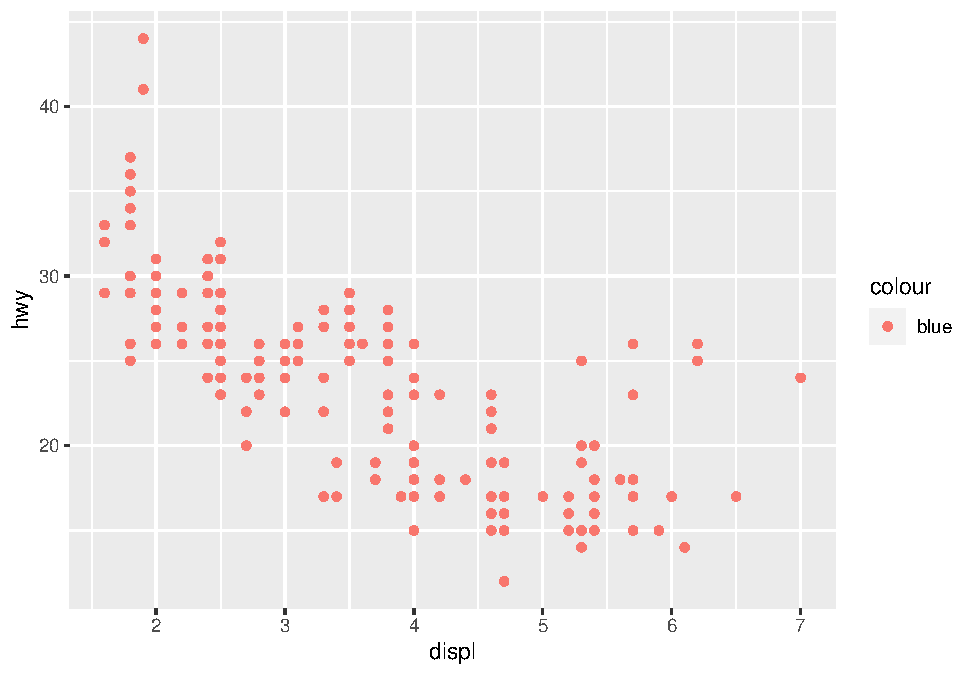
\includegraphics{r4dsexercises_files/figure-latex/3.3.1 Question 1-1.pdf}

\begin{Shaded}
\begin{Highlighting}[]
\CommentTok{#this is incorrect because there is a missing parenthesis after hwy. should be:}

\KeywordTok{ggplot}\NormalTok{(}\DataTypeTok{data =}\NormalTok{ mpg) }\OperatorTok{+}\StringTok{ }
\StringTok{  }\KeywordTok{geom_point}\NormalTok{(}\DataTypeTok{mapping =} \KeywordTok{aes}\NormalTok{(}\DataTypeTok{x =}\NormalTok{ displ, }\DataTypeTok{y =}\NormalTok{ hwy), }\DataTypeTok{color =} \StringTok{"blue"}\NormalTok{)}
\end{Highlighting}
\end{Shaded}

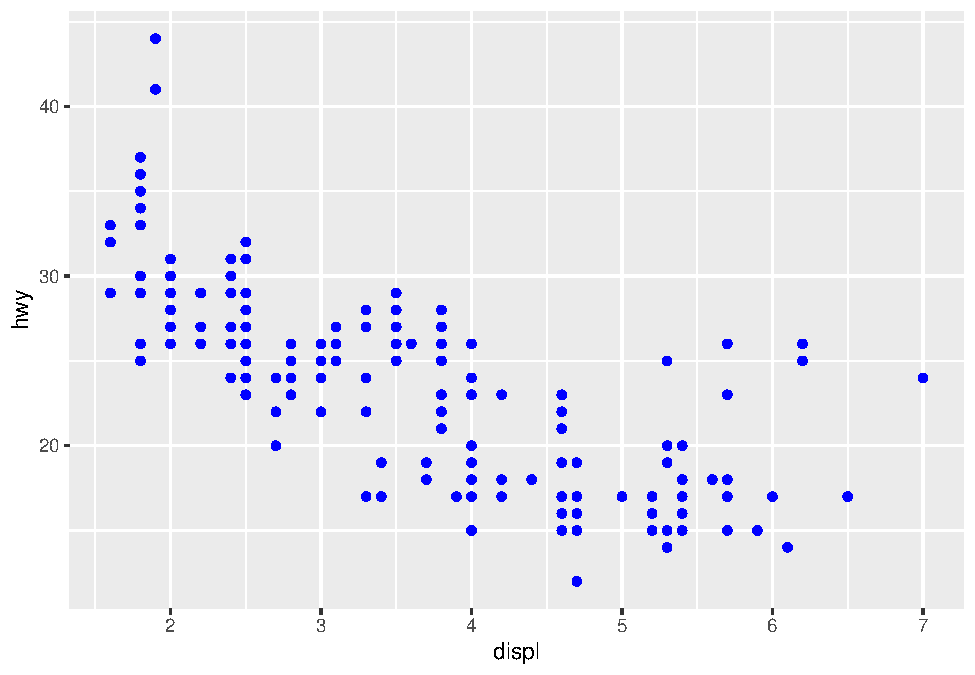
\includegraphics{r4dsexercises_files/figure-latex/3.3.1 Question 1-2.pdf}

\hypertarget{question-2which-variables-in-mpg-are-categorical-which-variables-are-continuous-hint-type-mpg-to-read-the-documentation-for-the-dataset.-how-can-you-see-this-information-when-you-run-mpg}{%
\subsection{Question 2:Which variables in mpg are categorical? Which variables are continuous? (Hint: type ?mpg to read the documentation for the dataset). How can you see this information when you run mpg?}\label{question-2which-variables-in-mpg-are-categorical-which-variables-are-continuous-hint-type-mpg-to-read-the-documentation-for-the-dataset.-how-can-you-see-this-information-when-you-run-mpg}}

categorical variables: manufacturer, model, trans, drv, fl, class
continuous variables: displ, year, cyl, cty, hwy

you can see this when you run mpg under the columns where it displays the type of variable (cat = cont = , )

\hypertarget{question-3map-a-continuous-variable-to-color-size-and-shape.-how-do-these-aesthetics-behave-differently-for-categorical-vs.-continuous-variables}{%
\subsection{Question 3:Map a continuous variable to color, size, and shape. How do these aesthetics behave differently for categorical vs.~continuous variables?}\label{question-3map-a-continuous-variable-to-color-size-and-shape.-how-do-these-aesthetics-behave-differently-for-categorical-vs.-continuous-variables}}

\begin{Shaded}
\begin{Highlighting}[]
\KeywordTok{ggplot}\NormalTok{(}\DataTypeTok{data =}\NormalTok{ mpg) }\OperatorTok{+}\StringTok{ }
\StringTok{  }\KeywordTok{geom_point}\NormalTok{(}\DataTypeTok{mapping =} \KeywordTok{aes}\NormalTok{(}\DataTypeTok{x =}\NormalTok{ displ, }\DataTypeTok{y =}\NormalTok{ hwy, }\DataTypeTok{size =}\NormalTok{ displ, }\DataTypeTok{color =}\NormalTok{ year, }\DataTypeTok{shape =}\NormalTok{ cyl))}
\end{Highlighting}
\end{Shaded}

\begin{verbatim}
## Error: A continuous variable can not be mapped to shape
\end{verbatim}


\includegraphics{r4dsexercises_files/figure-latex/3.3.1 Question 3.1-1.pdf}

you can't map a continuous variable to shape

\begin{Shaded}
\begin{Highlighting}[]
\KeywordTok{ggplot}\NormalTok{(}\DataTypeTok{data =}\NormalTok{ mpg) }\OperatorTok{+}
\StringTok{  }\KeywordTok{geom_point}\NormalTok{(}\DataTypeTok{mapping =} \KeywordTok{aes}\NormalTok{(}\DataTypeTok{x =}\NormalTok{ manufacturer, }\DataTypeTok{y =}\NormalTok{ model, }\DataTypeTok{size =}\NormalTok{ model, }\DataTypeTok{color =}\NormalTok{ trans, }\DataTypeTok{shape =}\NormalTok{ class))}
\end{Highlighting}
\end{Shaded}

\begin{verbatim}
## Warning: Using size for a discrete variable is not advised.
\end{verbatim}

\begin{verbatim}
## Warning: The shape palette can deal with a maximum of 6 discrete values because more than 6 becomes difficult to
## discriminate; you have 7. Consider specifying shapes manually if you must have them.
\end{verbatim}

\begin{verbatim}
## Warning: Removed 62 rows containing missing values (geom_point).
\end{verbatim}

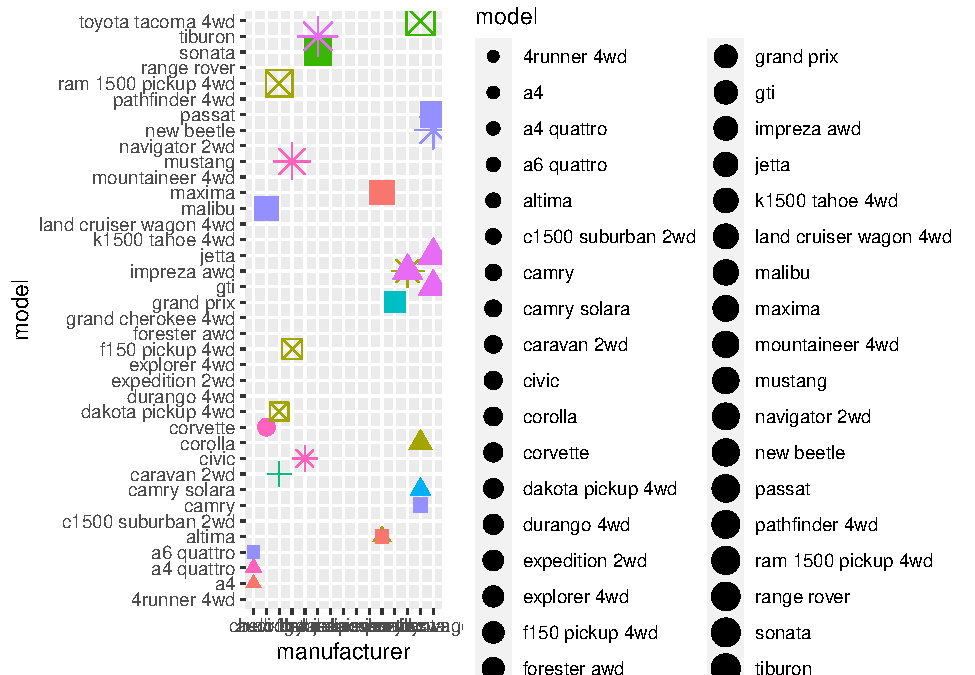
\includegraphics{r4dsexercises_files/figure-latex/3.3.1 Question 3.2-1.pdf}

You shouldn't use size for a discrete variable; the shape palette can only handle 6 values so any more doesn't work well; asks you to specify shapes if you have to have them.

\hypertarget{question-4-what-happens-if-you-map-the-same-variable-to-multiple-aesthetics}{%
\subsection{Question 4: What happens if you map the same variable to multiple aesthetics?}\label{question-4-what-happens-if-you-map-the-same-variable-to-multiple-aesthetics}}

The points for what you are graphing each have a specific color, size, and shape.

\begin{Shaded}
\begin{Highlighting}[]
\KeywordTok{ggplot}\NormalTok{(}\DataTypeTok{data =}\NormalTok{ mpg) }\OperatorTok{+}
\StringTok{  }\KeywordTok{geom_point}\NormalTok{(}\DataTypeTok{mapping =} \KeywordTok{aes}\NormalTok{(}\DataTypeTok{x =}\NormalTok{ manufacturer, }\DataTypeTok{y =}\NormalTok{ model, }\DataTypeTok{size =}\NormalTok{ class, }\DataTypeTok{color =}\NormalTok{ class, }\DataTypeTok{shape =}\NormalTok{ class))}
\end{Highlighting}
\end{Shaded}

\begin{verbatim}
## Warning: Using size for a discrete variable is not advised.
\end{verbatim}

\begin{verbatim}
## Warning: The shape palette can deal with a maximum of 6 discrete values because more than 6 becomes difficult to
## discriminate; you have 7. Consider specifying shapes manually if you must have them.
\end{verbatim}

\begin{verbatim}
## Warning: Removed 62 rows containing missing values (geom_point).
\end{verbatim}

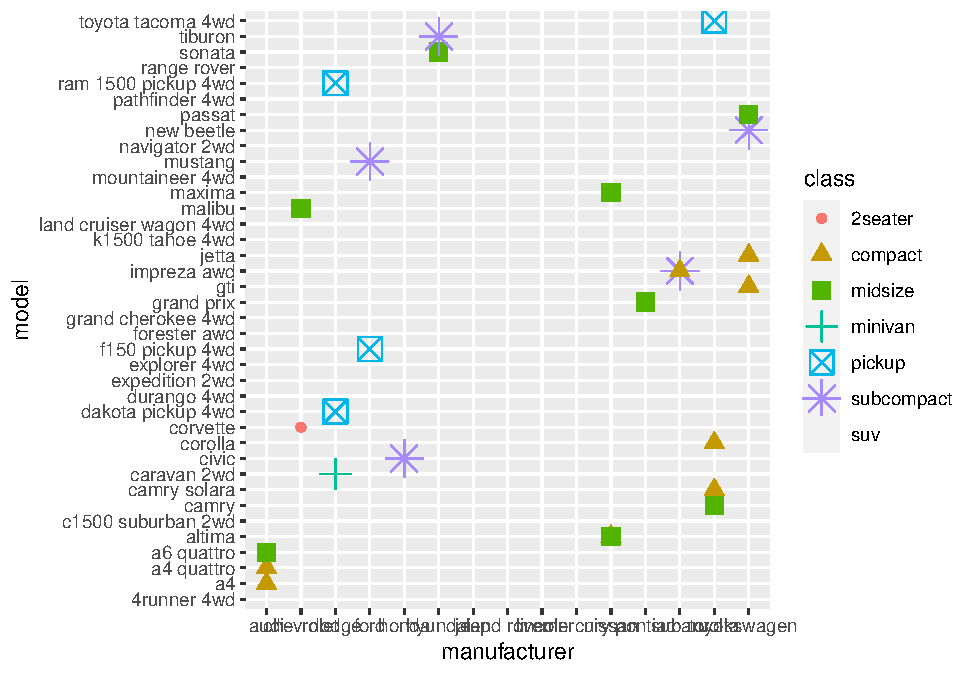
\includegraphics{r4dsexercises_files/figure-latex/3.3.1 Question 4-1.pdf}

\hypertarget{question-5-what-does-the-stroke-aesthetic-do-what-shapes-does-it-work-with-hint-use-geom_point}{%
\subsection{Question 5: What does the stroke aesthetic do? What shapes does it work with? (Hint: use ?geom\_point)}\label{question-5-what-does-the-stroke-aesthetic-do-what-shapes-does-it-work-with-hint-use-geom_point}}

if a shape had a border, stroke would control the width of the border

\hypertarget{question-6-what-happens-if-you-map-an-aesthetic-to-something-other-than-a-variable-name-like-aescolour-displ-5-note-youll-also-need-to-specify-x-and-y.}{%
\subsection{Question 6: What happens if you map an aesthetic to something other than a variable name, like aes(colour = displ \textless{} 5)? Note, you'll also need to specify x and y.}\label{question-6-what-happens-if-you-map-an-aesthetic-to-something-other-than-a-variable-name-like-aescolour-displ-5-note-youll-also-need-to-specify-x-and-y.}}

\begin{Shaded}
\begin{Highlighting}[]
\KeywordTok{ggplot}\NormalTok{(}\DataTypeTok{data =}\NormalTok{ mpg) }\OperatorTok{+}
\StringTok{  }\KeywordTok{geom_point}\NormalTok{(}\DataTypeTok{mapping =} \KeywordTok{aes}\NormalTok{(}\DataTypeTok{x =}\NormalTok{ manufacturer, }\DataTypeTok{y =}\NormalTok{ model, }\DataTypeTok{color =}\NormalTok{ displ }\OperatorTok{<}\StringTok{ }\DecValTok{5}\NormalTok{))}
\end{Highlighting}
\end{Shaded}

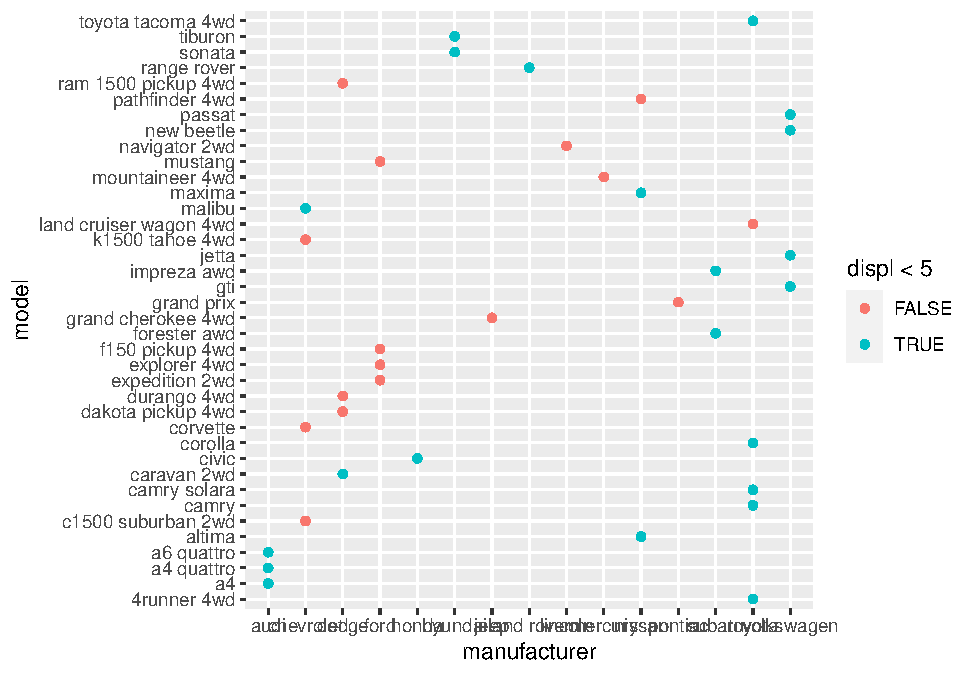
\includegraphics{r4dsexercises_files/figure-latex/3.3.1 Question 6-1.pdf}

This colors the points based on if the condition displ \textless{} 5 is true or false

\hypertarget{chapter-3.5.1-exercises}{%
\section{Chapter 3.5.1 Exercises}\label{chapter-3.5.1-exercises}}

\hypertarget{question-1-what-happens-if-you-facet-on-a-continuous-variable}{%
\subsection{Question 1: What happens if you facet on a continuous variable?}\label{question-1-what-happens-if-you-facet-on-a-continuous-variable}}

Creates a new graph for each of the numbers in the continuous variable like displ, see below

\begin{Shaded}
\begin{Highlighting}[]
\KeywordTok{ggplot}\NormalTok{(}\DataTypeTok{data =}\NormalTok{ mpg) }\OperatorTok{+}\StringTok{ }
\StringTok{  }\KeywordTok{geom_point}\NormalTok{(}\DataTypeTok{mapping =} \KeywordTok{aes}\NormalTok{(}\DataTypeTok{x =}\NormalTok{ displ, }\DataTypeTok{y =}\NormalTok{ hwy)) }\OperatorTok{+}\StringTok{ }
\StringTok{  }\KeywordTok{facet_wrap}\NormalTok{(}\OperatorTok{~}\StringTok{ }\NormalTok{displ, }\DataTypeTok{nrow =} \DecValTok{2}\NormalTok{)}
\end{Highlighting}
\end{Shaded}

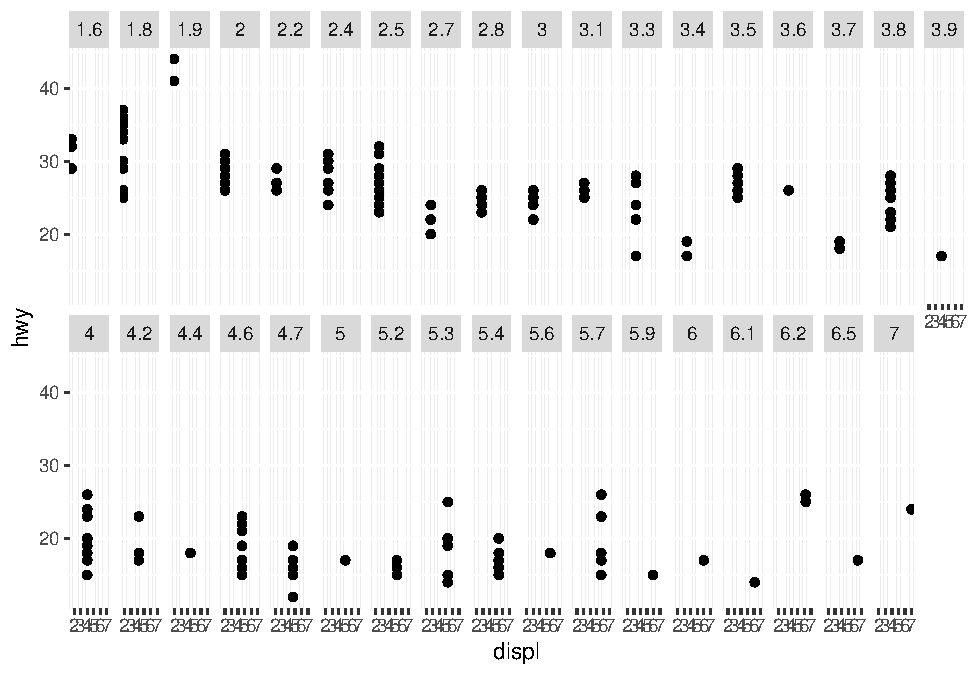
\includegraphics{r4dsexercises_files/figure-latex/3.5.1 Question 1-1.pdf}

\hypertarget{question-2-what-happens-if-you-facet-on-a-continuous-variable}{%
\subsection{Question 2: What happens if you facet on a continuous variable?}\label{question-2-what-happens-if-you-facet-on-a-continuous-variable}}

The empty cells in the plot with facet\_grid(drv \textasciitilde{} cyl) show that there are no points that relate to both variables (cyl, drv). for example, for the cells with 5 cylinders and 4wd, there are no points so cannot plot the displ and hwy for it.

\begin{Shaded}
\begin{Highlighting}[]
\KeywordTok{ggplot}\NormalTok{(}\DataTypeTok{data =}\NormalTok{ mpg) }\OperatorTok{+}\StringTok{ }
\StringTok{  }\KeywordTok{geom_point}\NormalTok{(}\DataTypeTok{mapping =} \KeywordTok{aes}\NormalTok{(}\DataTypeTok{x =}\NormalTok{ displ, }\DataTypeTok{y =}\NormalTok{ hwy)) }\OperatorTok{+}\StringTok{ }
\StringTok{  }\KeywordTok{facet_grid}\NormalTok{(drv }\OperatorTok{~}\StringTok{ }\NormalTok{cyl)}
\end{Highlighting}
\end{Shaded}

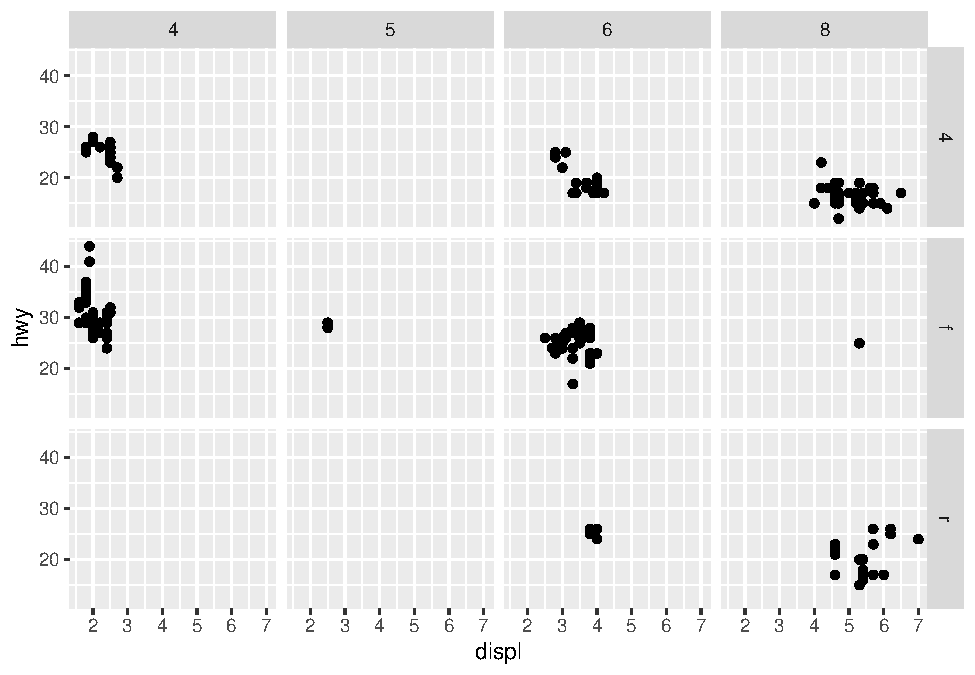
\includegraphics{r4dsexercises_files/figure-latex/3.5.1 Question 2-1.pdf}

\hypertarget{question-3-what-plots-does-the-following-code-make-what-does-.-do}{%
\subsection{Question 3: What plots does the following code make? What does . do?}\label{question-3-what-plots-does-the-following-code-make-what-does-.-do}}

The `.' determines where the drv axis will be (on the righthand side vs the top). It is the placeholder for the empty axis.

\begin{Shaded}
\begin{Highlighting}[]
\KeywordTok{ggplot}\NormalTok{(}\DataTypeTok{data =}\NormalTok{ mpg) }\OperatorTok{+}\StringTok{ }
\StringTok{  }\KeywordTok{geom_point}\NormalTok{(}\DataTypeTok{mapping =} \KeywordTok{aes}\NormalTok{(}\DataTypeTok{x =}\NormalTok{ displ, }\DataTypeTok{y =}\NormalTok{ hwy)) }\OperatorTok{+}
\StringTok{  }\KeywordTok{facet_grid}\NormalTok{(drv }\OperatorTok{~}\StringTok{ }\NormalTok{.) }
\end{Highlighting}
\end{Shaded}

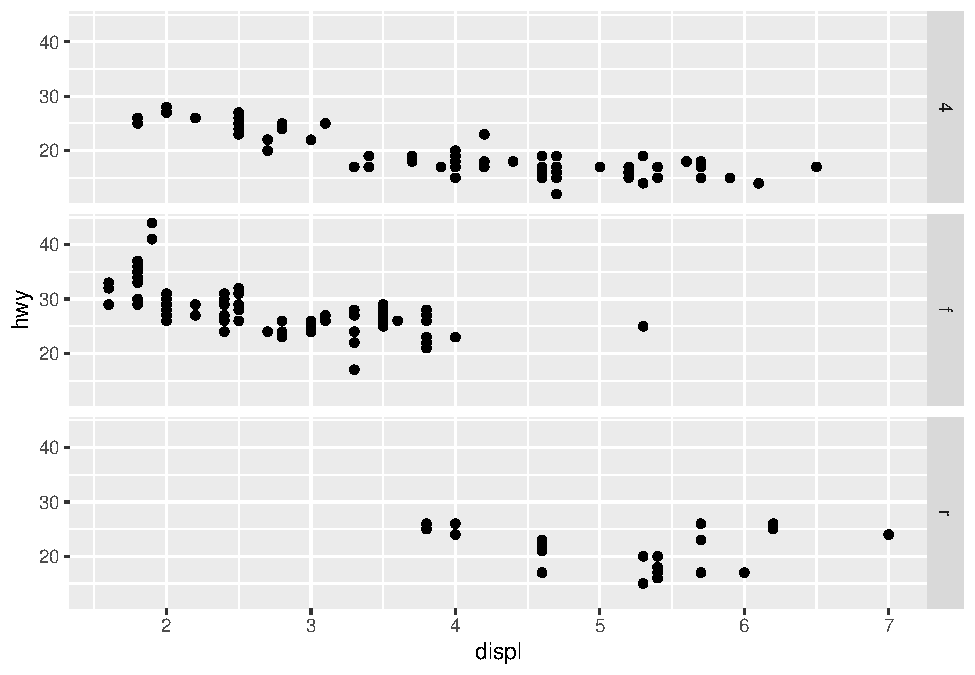
\includegraphics{r4dsexercises_files/figure-latex/3.5.1 Question 3-1.pdf}

\begin{Shaded}
\begin{Highlighting}[]
\KeywordTok{ggplot}\NormalTok{(}\DataTypeTok{data =}\NormalTok{ mpg) }\OperatorTok{+}\StringTok{ }
\StringTok{  }\KeywordTok{geom_point}\NormalTok{(}\DataTypeTok{mapping =} \KeywordTok{aes}\NormalTok{(}\DataTypeTok{x =}\NormalTok{ displ, }\DataTypeTok{y =}\NormalTok{ hwy)) }\OperatorTok{+}
\StringTok{  }\KeywordTok{facet_grid}\NormalTok{(. }\OperatorTok{~}\StringTok{ }\NormalTok{drv) }
\end{Highlighting}
\end{Shaded}

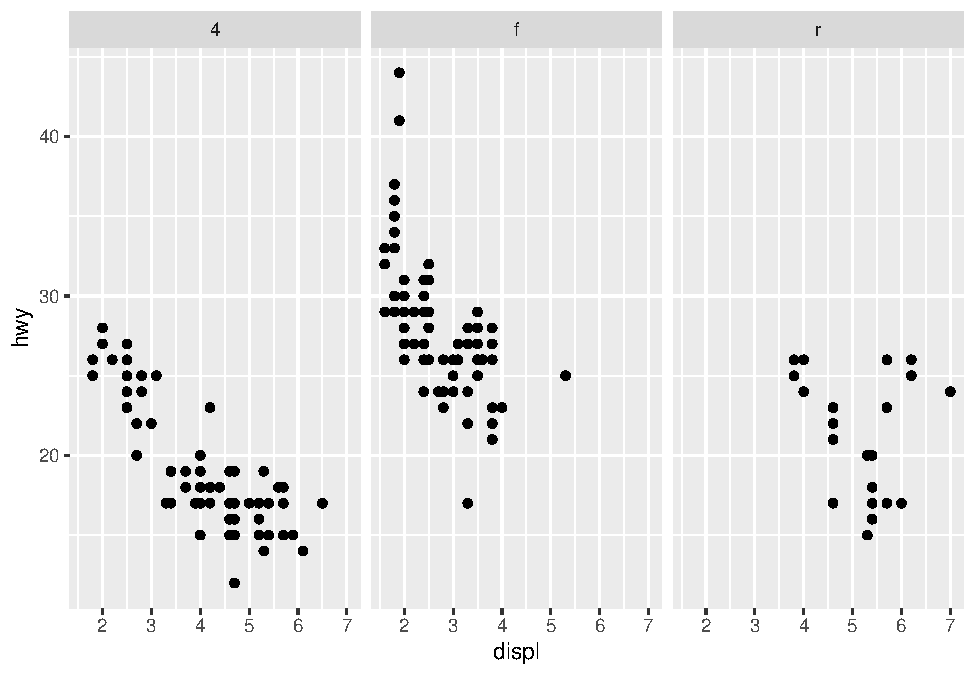
\includegraphics{r4dsexercises_files/figure-latex/3.5.1 Question 3-2.pdf}

\hypertarget{question-4-take-the-first-faceted-plot-in-this-section.-what-are-the-advantages-to-using-faceting-instead-of-the-colour-aesthetic-what-are-the-disadvantages-how-might-the-balance-change-if-you-had-a-larger-dataset}{%
\subsection{Question 4: Take the first faceted plot in this section. What are the advantages to using faceting instead of the colour aesthetic? What are the disadvantages? How might the balance change if you had a larger dataset?}\label{question-4-take-the-first-faceted-plot-in-this-section.-what-are-the-advantages-to-using-faceting-instead-of-the-colour-aesthetic-what-are-the-disadvantages-how-might-the-balance-change-if-you-had-a-larger-dataset}}

The advantage of using facet wrap instead of color is that it allows you to more easily see differences in hwy and displ for each car type because they are separated into individual graphs. Especially for large datasets, it would be quite difficult to see all of one car types' data points with color because they could overlap on the graph.

\begin{Shaded}
\begin{Highlighting}[]
\KeywordTok{ggplot}\NormalTok{(}\DataTypeTok{data =}\NormalTok{ mpg) }\OperatorTok{+}\StringTok{ }
\StringTok{  }\KeywordTok{geom_point}\NormalTok{(}\DataTypeTok{mapping =} \KeywordTok{aes}\NormalTok{(}\DataTypeTok{x =}\NormalTok{ displ, }\DataTypeTok{y =}\NormalTok{ hwy)) }\OperatorTok{+}\StringTok{ }
\StringTok{  }\KeywordTok{facet_wrap}\NormalTok{(}\OperatorTok{~}\StringTok{ }\NormalTok{class, }\DataTypeTok{nrow =} \DecValTok{2}\NormalTok{)}
\end{Highlighting}
\end{Shaded}

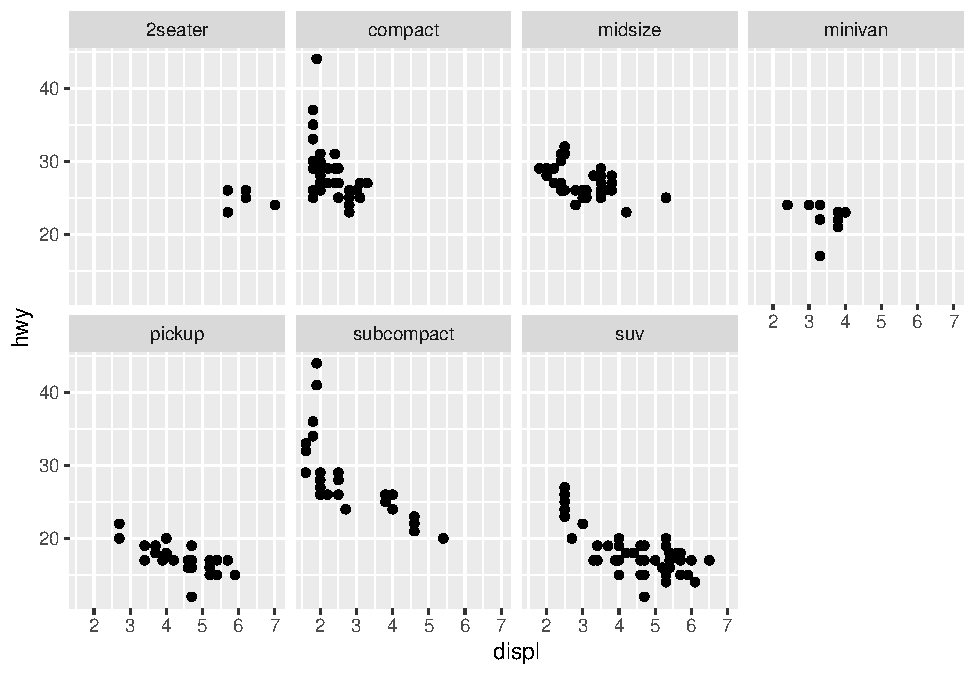
\includegraphics{r4dsexercises_files/figure-latex/3.5.1 Question 4-1.pdf}

\hypertarget{question-5-read-facet_wrap.-what-does-nrow-do-what-does-ncol-do-what-other-options-control-the-layout-of-the-individual-panels-why-doesnt-facet_grid-have-nrow-and-ncol-arguments}{%
\subsection{Question 5: Read ?facet\_wrap. What does nrow do? What does ncol do? What other options control the layout of the individual panels? Why doesn't facet\_grid() have nrow and ncol arguments?}\label{question-5-read-facet_wrap.-what-does-nrow-do-what-does-ncol-do-what-other-options-control-the-layout-of-the-individual-panels-why-doesnt-facet_grid-have-nrow-and-ncol-arguments}}

nrow is the number of rows, ncol is the number of columns. The other options that control the layout of the panels include: scales, shrink, switch, dir, strip.position. Facet\_grid does not have nrow and ncol because it is creating a matrix of panels, and does not on its own have a specified number of columns and rows.

\hypertarget{question-6-when-using-facet_grid-you-should-usually-put-the-variable-with-more-unique-levels-in-the-columns.-why}{%
\subsection{Question 6: When using facet\_grid() you should usually put the variable with more unique levels in the columns. Why?}\label{question-6-when-using-facet_grid-you-should-usually-put-the-variable-with-more-unique-levels-in-the-columns.-why}}

Because if you add more levels to the rows, the col axis (y-axis) would be shorter, meaning that it would be harder to see the actual values on the plots.

\hypertarget{chapter-3.6.1-excersises}{%
\section{Chapter 3.6.1 Excersises}\label{chapter-3.6.1-excersises}}

\hypertarget{question-1-what-geom-would-you-use-to-draw-a-line-chart-a-boxplot-a-histogram-an-area-chart}{%
\subsection{Question 1: What geom would you use to draw a line chart? A boxplot? A histogram? An area chart?}\label{question-1-what-geom-would-you-use-to-draw-a-line-chart-a-boxplot-a-histogram-an-area-chart}}

line chart: geom\_smooth
boxplot: geom\_boxplot
histogram: geom\_histogram
area chart: geom\_area

\hypertarget{question-2-run-this-code-in-your-head-and-predict-what-the-output-will-look-like.-then-run-the-code-in-r-and-check-your-predictions.}{%
\subsection{Question 2: Run this code in your head and predict what the output will look like. Then, run the code in R and check your predictions.}\label{question-2-run-this-code-in-your-head-and-predict-what-the-output-will-look-like.-then-run-the-code-in-r-and-check-your-predictions.}}

\begin{Shaded}
\begin{Highlighting}[]
\KeywordTok{ggplot}\NormalTok{(}\DataTypeTok{data =}\NormalTok{ mpg, }\DataTypeTok{mapping =} \KeywordTok{aes}\NormalTok{(}\DataTypeTok{x =}\NormalTok{ displ, }\DataTypeTok{y =}\NormalTok{ hwy, }\DataTypeTok{color =}\NormalTok{ drv)) }\OperatorTok{+}\StringTok{ }
\StringTok{  }\KeywordTok{geom_point}\NormalTok{() }\OperatorTok{+}\StringTok{ }
\StringTok{  }\KeywordTok{geom_smooth}\NormalTok{(}\DataTypeTok{se =} \OtherTok{FALSE}\NormalTok{)}
\end{Highlighting}
\end{Shaded}

\begin{verbatim}
## `geom_smooth()` using method = 'loess' and formula 'y ~ x'
\end{verbatim}

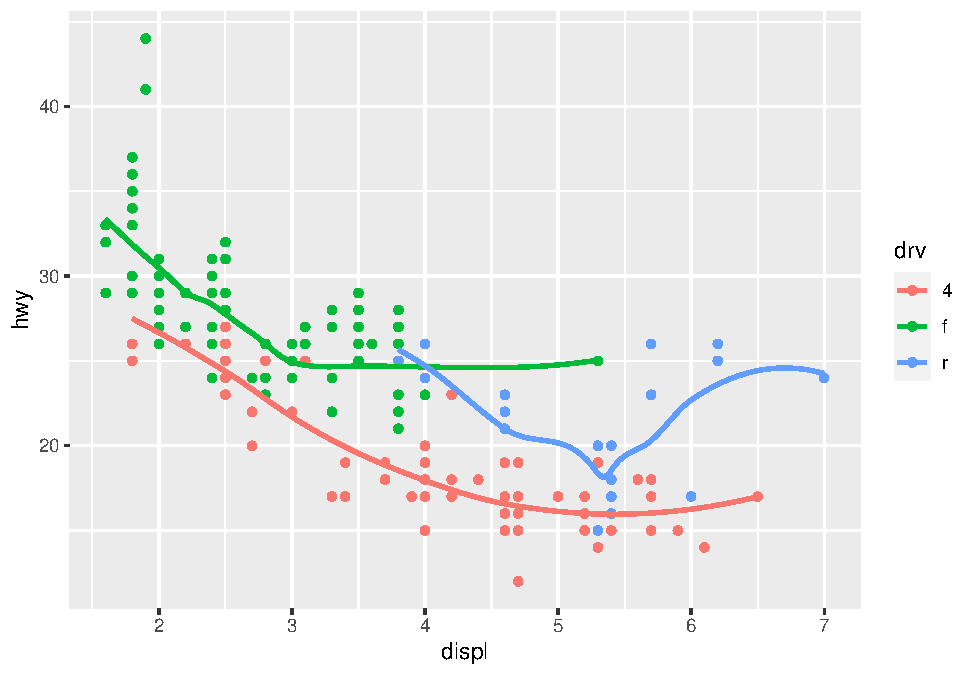
\includegraphics{r4dsexercises_files/figure-latex/3.6.1 Question 2-1.pdf}

\hypertarget{question-3-what-does-show.legend-false-do-what-happens-if-you-remove-it}{%
\subsection{Question 3: What does show.legend = FALSE do? What happens if you remove it?}\label{question-3-what-does-show.legend-false-do-what-happens-if-you-remove-it}}

show.legend = FALSE will remove the legend key from the plot. If it is not there, the ggplot function assumes it should exist to describe the aesthetics for variables.

\hypertarget{question-4-what-does-the-se-argument-to-geom_smooth-do}{%
\subsection{Question 4: What does the se argument to geom\_smooth() do?}\label{question-4-what-does-the-se-argument-to-geom_smooth-do}}

se shows the confidence interval around the smooth line

\hypertarget{question-5-will-these-two-graphs-look-different-whywhy-not}{%
\subsection{Question 5: Will these two graphs look different? Why/why not?}\label{question-5-will-these-two-graphs-look-different-whywhy-not}}

\begin{Shaded}
\begin{Highlighting}[]
\KeywordTok{ggplot}\NormalTok{(}\DataTypeTok{data =}\NormalTok{ mpg, }\DataTypeTok{mapping =} \KeywordTok{aes}\NormalTok{(}\DataTypeTok{x =}\NormalTok{ displ, }\DataTypeTok{y =}\NormalTok{ hwy)) }\OperatorTok{+}\StringTok{ }
\StringTok{  }\KeywordTok{geom_point}\NormalTok{() }\OperatorTok{+}\StringTok{ }
\StringTok{  }\KeywordTok{geom_smooth}\NormalTok{()}
\end{Highlighting}
\end{Shaded}

\begin{verbatim}
## `geom_smooth()` using method = 'loess' and formula 'y ~ x'
\end{verbatim}

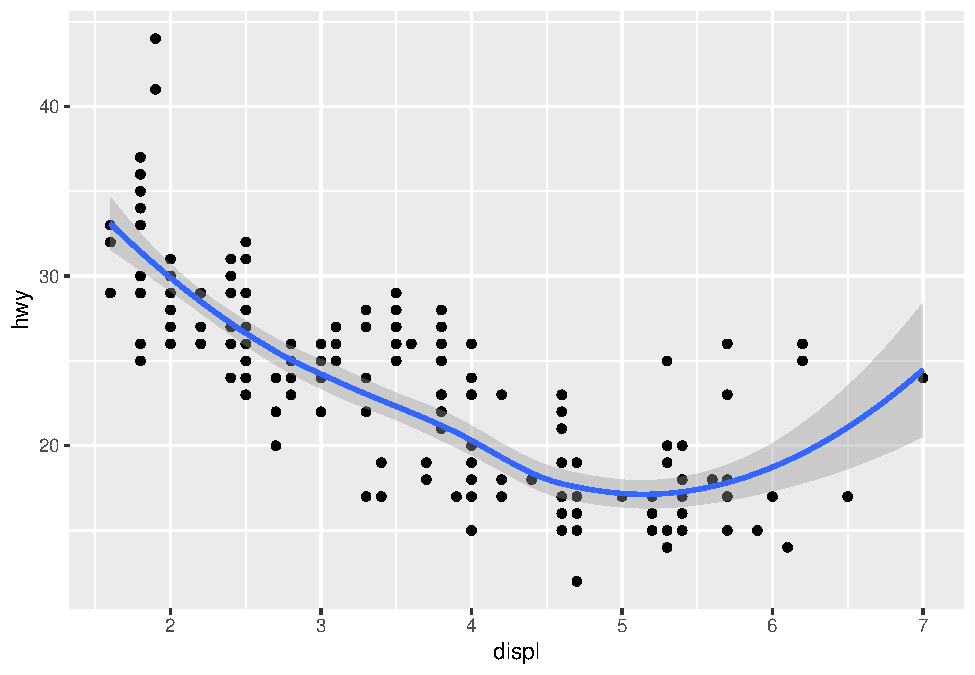
\includegraphics{r4dsexercises_files/figure-latex/3.6.1 Question 5-1.pdf}

\begin{Shaded}
\begin{Highlighting}[]
\KeywordTok{ggplot}\NormalTok{() }\OperatorTok{+}\StringTok{ }
\StringTok{  }\KeywordTok{geom_point}\NormalTok{(}\DataTypeTok{data =}\NormalTok{ mpg, }\DataTypeTok{mapping =} \KeywordTok{aes}\NormalTok{(}\DataTypeTok{x =}\NormalTok{ displ, }\DataTypeTok{y =}\NormalTok{ hwy)) }\OperatorTok{+}\StringTok{ }
\StringTok{  }\KeywordTok{geom_smooth}\NormalTok{(}\DataTypeTok{data =}\NormalTok{ mpg, }\DataTypeTok{mapping =} \KeywordTok{aes}\NormalTok{(}\DataTypeTok{x =}\NormalTok{ displ, }\DataTypeTok{y =}\NormalTok{ hwy))}
\end{Highlighting}
\end{Shaded}

\begin{verbatim}
## `geom_smooth()` using method = 'loess' and formula 'y ~ x'
\end{verbatim}

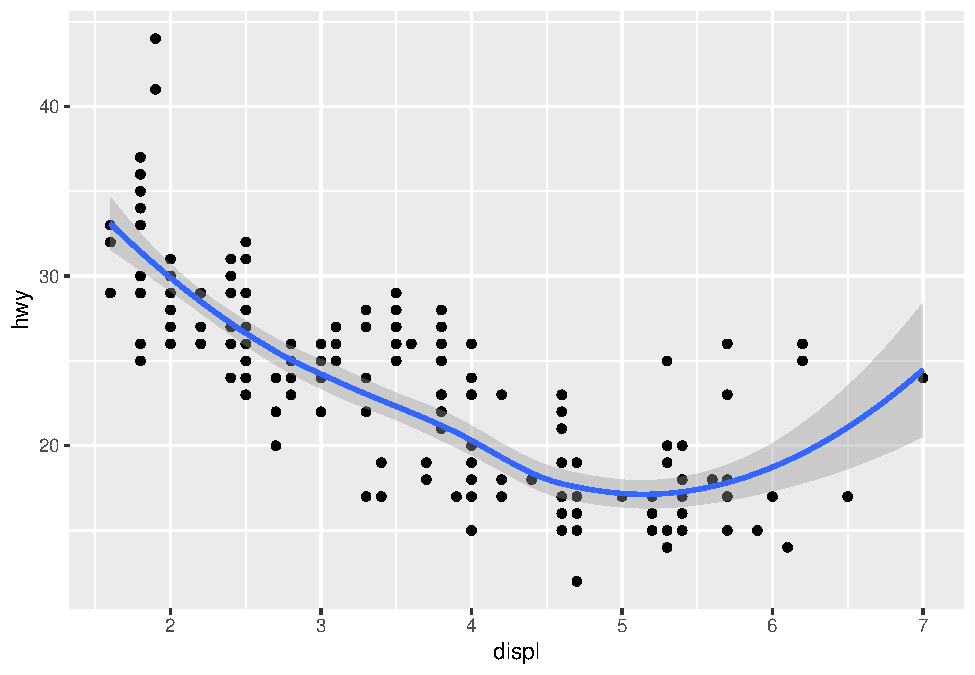
\includegraphics{r4dsexercises_files/figure-latex/3.6.1 Question 5-2.pdf}

These graphs don't look different because they are identical in meaning. The top code is much more concise code, as the data and aesthetics are described in the ggplot portion and the point and smooth functions are how the data will plot.

\hypertarget{question-6-recreate-the-r-code-necessary-to-generate-the-following-graphs.}{%
\subsection{Question 6: Recreate the R code necessary to generate the following graphs.}\label{question-6-recreate-the-r-code-necessary-to-generate-the-following-graphs.}}

\begin{Shaded}
\begin{Highlighting}[]
\KeywordTok{ggplot}\NormalTok{(}\DataTypeTok{data =}\NormalTok{ mpg, }\DataTypeTok{mapping =} \KeywordTok{aes}\NormalTok{(}\DataTypeTok{x =}\NormalTok{ displ, }\DataTypeTok{y =}\NormalTok{ hwy)) }\OperatorTok{+}\StringTok{ }
\StringTok{  }\KeywordTok{geom_point}\NormalTok{() }\OperatorTok{+}\StringTok{ }
\StringTok{  }\KeywordTok{geom_smooth}\NormalTok{(}\DataTypeTok{se =} \OtherTok{FALSE}\NormalTok{)}
\end{Highlighting}
\end{Shaded}

\begin{verbatim}
## `geom_smooth()` using method = 'loess' and formula 'y ~ x'
\end{verbatim}

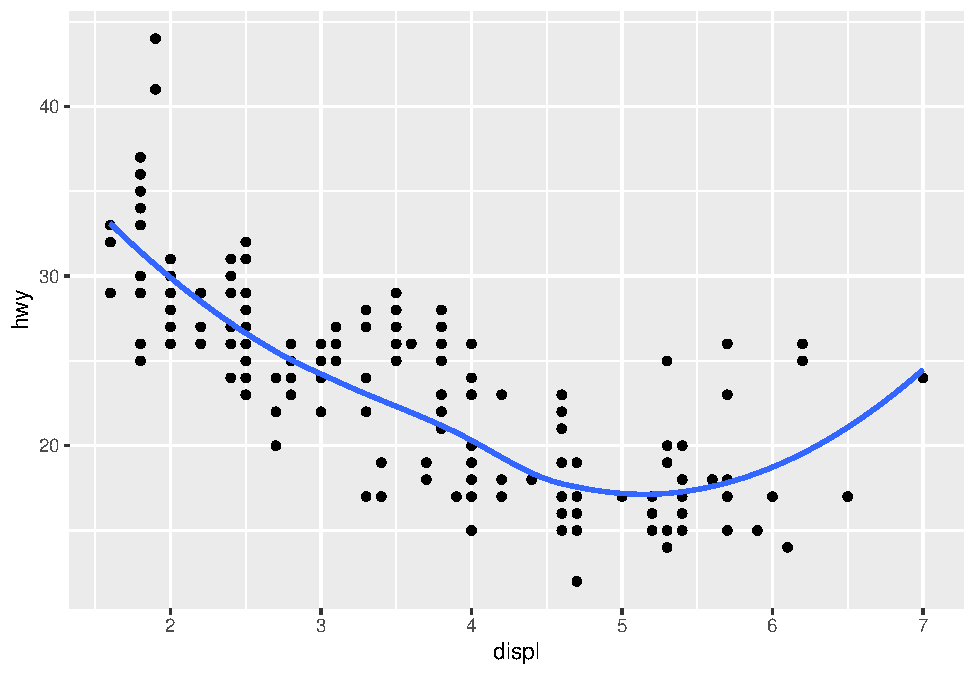
\includegraphics{r4dsexercises_files/figure-latex/3.6.1 Question 6-1.pdf}

\begin{Shaded}
\begin{Highlighting}[]
\KeywordTok{ggplot}\NormalTok{(}\DataTypeTok{data =}\NormalTok{ mpg, }\DataTypeTok{mapping =} \KeywordTok{aes}\NormalTok{(}\DataTypeTok{x =}\NormalTok{ displ, }\DataTypeTok{y =}\NormalTok{ hwy)) }\OperatorTok{+}\StringTok{ }
\StringTok{  }\KeywordTok{geom_point}\NormalTok{() }\OperatorTok{+}\StringTok{ }
\StringTok{  }\KeywordTok{geom_smooth}\NormalTok{(}\DataTypeTok{data =}\NormalTok{ mpg, }\DataTypeTok{mapping =} \KeywordTok{aes}\NormalTok{(}\DataTypeTok{x =}\NormalTok{ displ, }\DataTypeTok{y =}\NormalTok{ hwy, }\DataTypeTok{group =}\NormalTok{ drv), }\DataTypeTok{se =} \OtherTok{FALSE}\NormalTok{)}
\end{Highlighting}
\end{Shaded}

\begin{verbatim}
## `geom_smooth()` using method = 'loess' and formula 'y ~ x'
\end{verbatim}

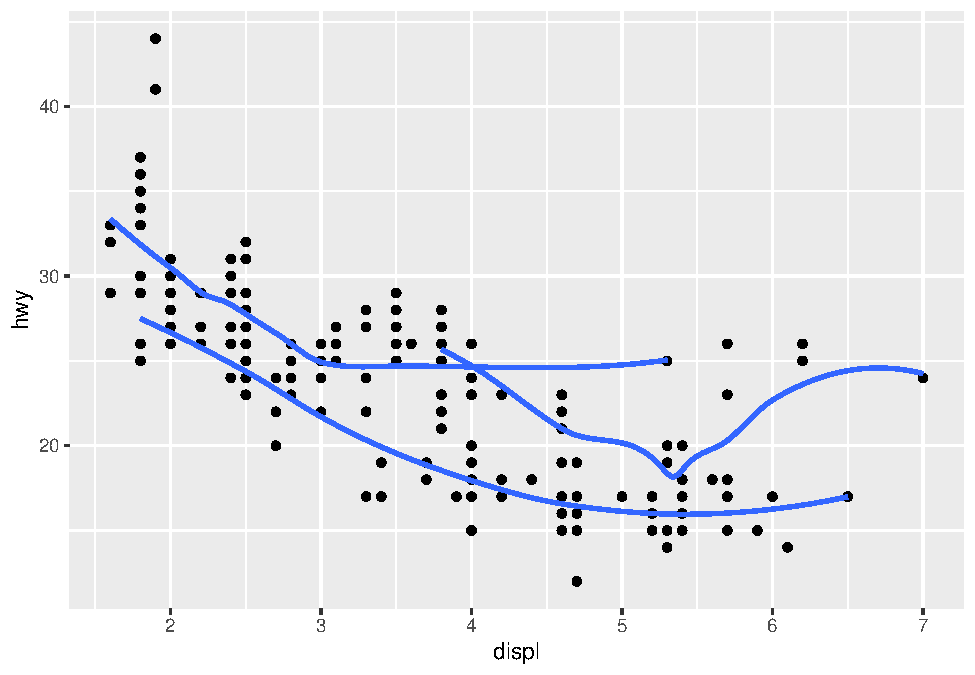
\includegraphics{r4dsexercises_files/figure-latex/3.6.1 Question 6-2.pdf}

\begin{Shaded}
\begin{Highlighting}[]
\KeywordTok{ggplot}\NormalTok{(}\DataTypeTok{data =}\NormalTok{ mpg, }\DataTypeTok{mapping =} \KeywordTok{aes}\NormalTok{(}\DataTypeTok{x =}\NormalTok{ displ, }\DataTypeTok{y =}\NormalTok{ hwy, }\DataTypeTok{color =}\NormalTok{ drv)) }\OperatorTok{+}\StringTok{ }
\StringTok{  }\KeywordTok{geom_point}\NormalTok{() }\OperatorTok{+}\StringTok{ }
\StringTok{  }\KeywordTok{geom_smooth}\NormalTok{(}\DataTypeTok{data =}\NormalTok{ mpg, }\DataTypeTok{mapping =} \KeywordTok{aes}\NormalTok{(}\DataTypeTok{x =}\NormalTok{ displ, }\DataTypeTok{y =}\NormalTok{ hwy, }\DataTypeTok{group =}\NormalTok{ drv), }\DataTypeTok{se =} \OtherTok{FALSE}\NormalTok{)}
\end{Highlighting}
\end{Shaded}

\begin{verbatim}
## `geom_smooth()` using method = 'loess' and formula 'y ~ x'
\end{verbatim}

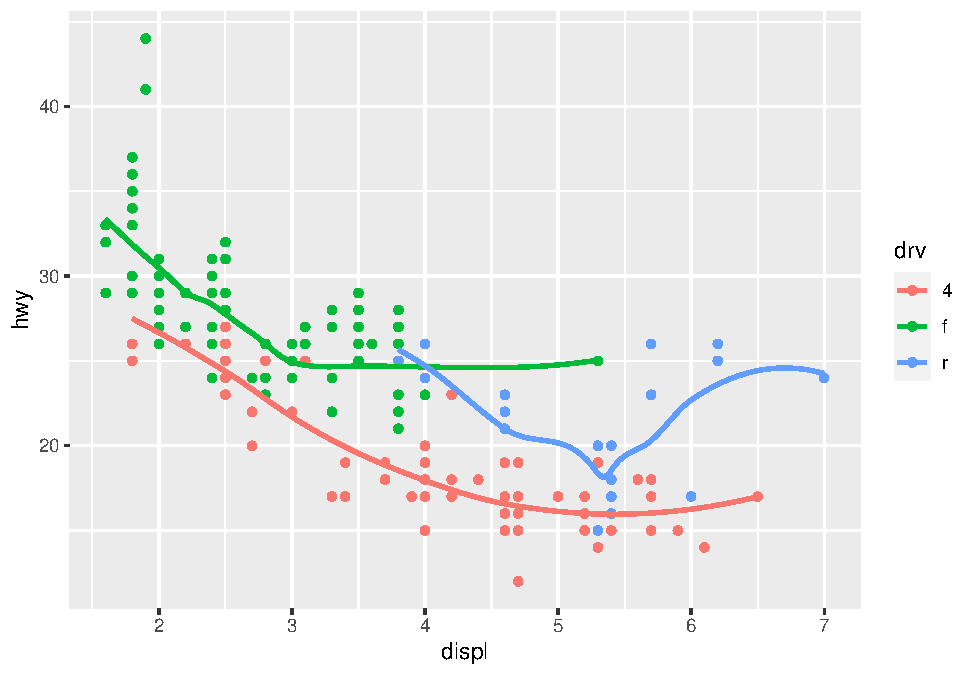
\includegraphics{r4dsexercises_files/figure-latex/3.6.1 Question 6-3.pdf}

\begin{Shaded}
\begin{Highlighting}[]
\KeywordTok{ggplot}\NormalTok{(}\DataTypeTok{data =}\NormalTok{ mpg, }\DataTypeTok{mapping =} \KeywordTok{aes}\NormalTok{(}\DataTypeTok{x =}\NormalTok{ displ, }\DataTypeTok{y =}\NormalTok{ hwy)) }\OperatorTok{+}\StringTok{ }
\StringTok{  }\KeywordTok{geom_point}\NormalTok{(}\DataTypeTok{mapping =} \KeywordTok{aes}\NormalTok{(}\DataTypeTok{color =}\NormalTok{ drv)) }\OperatorTok{+}\StringTok{ }
\StringTok{  }\KeywordTok{geom_smooth}\NormalTok{(}\DataTypeTok{se =} \OtherTok{FALSE}\NormalTok{)}
\end{Highlighting}
\end{Shaded}

\begin{verbatim}
## `geom_smooth()` using method = 'loess' and formula 'y ~ x'
\end{verbatim}

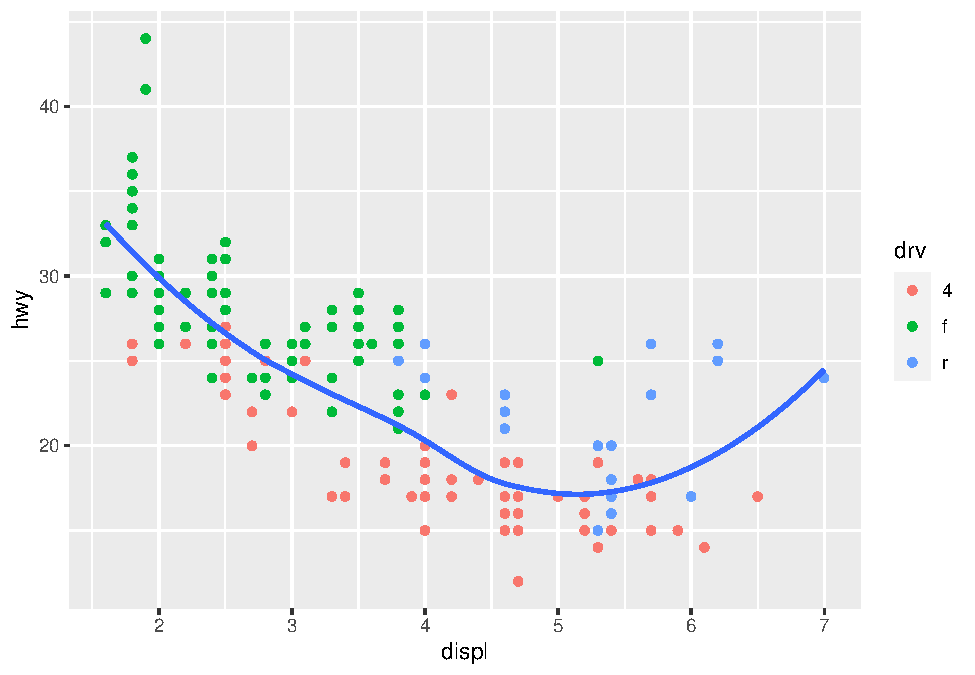
\includegraphics{r4dsexercises_files/figure-latex/3.6.1 Question 6-4.pdf}

\begin{Shaded}
\begin{Highlighting}[]
\KeywordTok{ggplot}\NormalTok{(}\DataTypeTok{data =}\NormalTok{ mpg, }\DataTypeTok{mapping =} \KeywordTok{aes}\NormalTok{(}\DataTypeTok{x =}\NormalTok{ displ, }\DataTypeTok{y =}\NormalTok{ hwy)) }\OperatorTok{+}\StringTok{ }
\StringTok{  }\KeywordTok{geom_point}\NormalTok{(}\DataTypeTok{mapping =} \KeywordTok{aes}\NormalTok{(}\DataTypeTok{color =}\NormalTok{ drv)) }\OperatorTok{+}\StringTok{ }
\StringTok{  }\KeywordTok{geom_smooth}\NormalTok{(}\DataTypeTok{se =} \OtherTok{FALSE}\NormalTok{)}
\end{Highlighting}
\end{Shaded}

\begin{verbatim}
## `geom_smooth()` using method = 'loess' and formula 'y ~ x'
\end{verbatim}

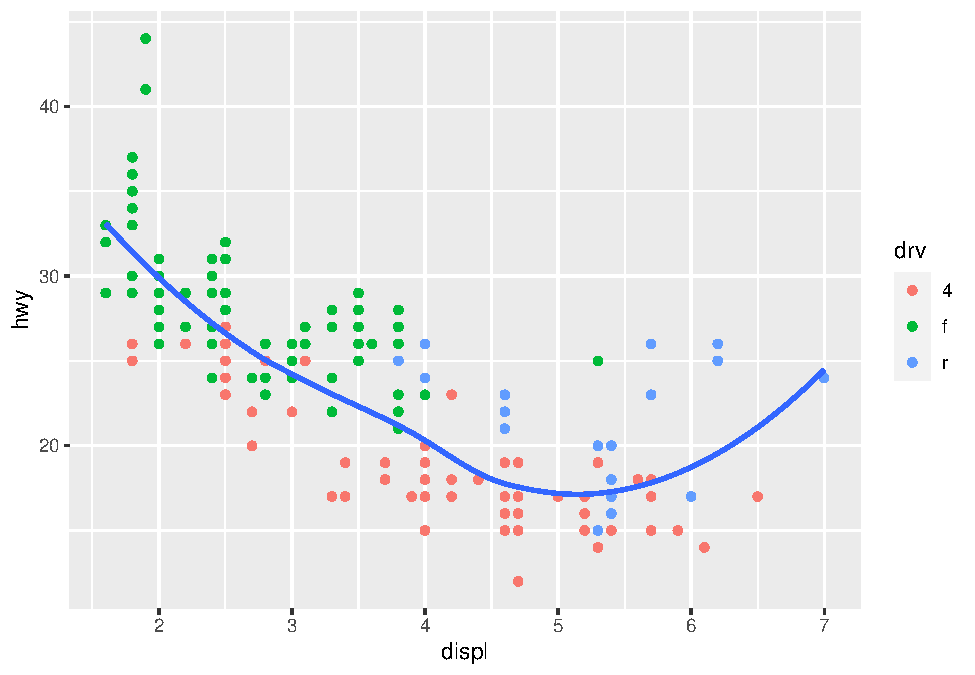
\includegraphics{r4dsexercises_files/figure-latex/3.6.1 Question 6-5.pdf}

\begin{Shaded}
\begin{Highlighting}[]
\KeywordTok{ggplot}\NormalTok{(}\DataTypeTok{data =}\NormalTok{ mpg, }\DataTypeTok{mapping =} \KeywordTok{aes}\NormalTok{(}\DataTypeTok{x =}\NormalTok{ displ, }\DataTypeTok{y =}\NormalTok{ hwy)) }\OperatorTok{+}\StringTok{ }
\StringTok{  }\KeywordTok{geom_point}\NormalTok{(}\DataTypeTok{mapping =} \KeywordTok{aes}\NormalTok{(}\DataTypeTok{color =}\NormalTok{ drv)) }\OperatorTok{+}\StringTok{ }
\StringTok{  }\KeywordTok{geom_smooth}\NormalTok{(}\DataTypeTok{mapping =} \KeywordTok{aes}\NormalTok{(}\DataTypeTok{x =}\NormalTok{ displ, }\DataTypeTok{y =}\NormalTok{ hwy, }\DataTypeTok{group =}\NormalTok{ drv), }\DataTypeTok{se =} \OtherTok{FALSE}\NormalTok{)}
\end{Highlighting}
\end{Shaded}

\begin{verbatim}
## `geom_smooth()` using method = 'loess' and formula 'y ~ x'
\end{verbatim}

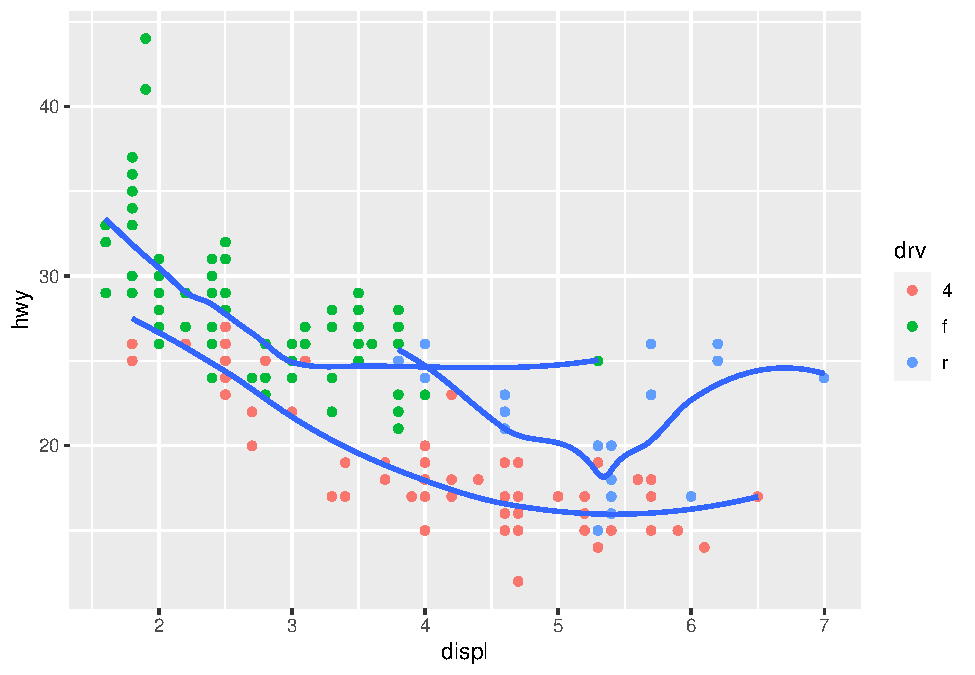
\includegraphics{r4dsexercises_files/figure-latex/3.6.1 Question 6-6.pdf}

\begin{Shaded}
\begin{Highlighting}[]
\KeywordTok{ggplot}\NormalTok{(}\DataTypeTok{data =}\NormalTok{ mpg, }\DataTypeTok{mapping =} \KeywordTok{aes}\NormalTok{(}\DataTypeTok{x =}\NormalTok{ displ, }\DataTypeTok{y =}\NormalTok{ hwy)) }\OperatorTok{+}
\StringTok{  }\KeywordTok{geom_point}\NormalTok{(}\DataTypeTok{colour =} \StringTok{"white"}\NormalTok{, }\DataTypeTok{size =} \DecValTok{4}\NormalTok{) }\OperatorTok{+}
\StringTok{  }\KeywordTok{geom_point}\NormalTok{(}\DataTypeTok{mapping =} \KeywordTok{aes}\NormalTok{(}\DataTypeTok{color =}\NormalTok{ drv), }\DataTypeTok{size =} \FloatTok{1.5}\NormalTok{)}
\end{Highlighting}
\end{Shaded}

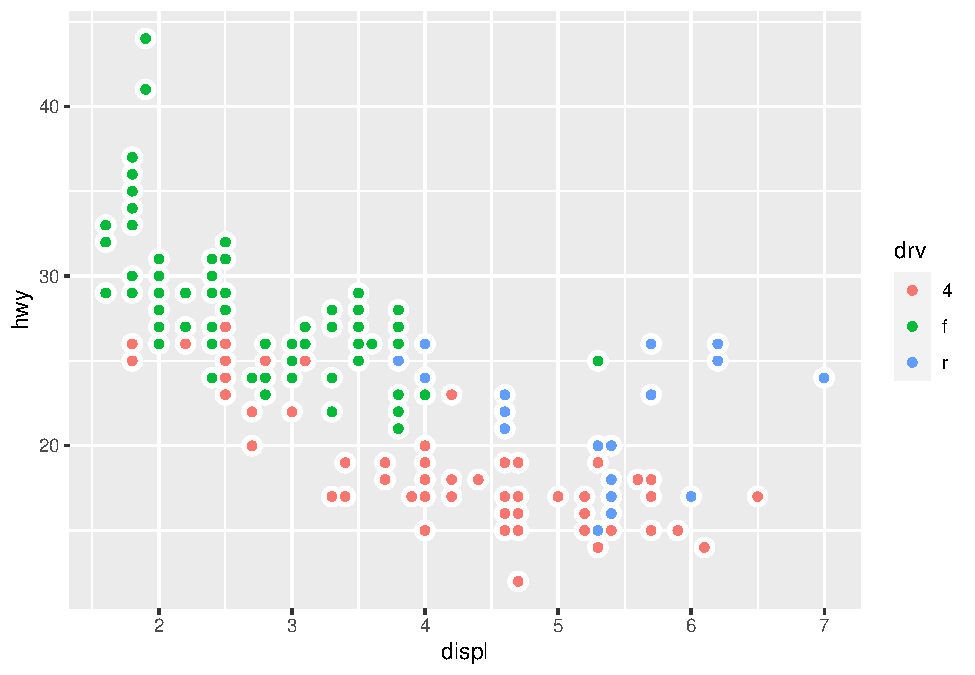
\includegraphics{r4dsexercises_files/figure-latex/3.6.1 Question 6-7.pdf}

\hypertarget{chapter-3.7.1-exercises}{%
\section{Chapter 3.7.1 Exercises}\label{chapter-3.7.1-exercises}}

\hypertarget{question-1-what-is-the-default-geom-associated-with-stat_summary-how-could-you-rewrite-the-previous-plot-to-use-that-geom-function-instead-of-the-stat-function}{%
\subsection{Question 1: What is the default geom associated with stat\_summary()? How could you rewrite the previous plot to use that geom function instead of the stat function?}\label{question-1-what-is-the-default-geom-associated-with-stat_summary-how-could-you-rewrite-the-previous-plot-to-use-that-geom-function-instead-of-the-stat-function}}

The default geom is pointrange.

\begin{Shaded}
\begin{Highlighting}[]
\KeywordTok{ggplot}\NormalTok{(}\DataTypeTok{data =}\NormalTok{ diamonds) }\OperatorTok{+}\StringTok{ }
\StringTok{  }\KeywordTok{stat_summary}\NormalTok{(}
    \DataTypeTok{mapping =} \KeywordTok{aes}\NormalTok{(}\DataTypeTok{x =}\NormalTok{ cut, }\DataTypeTok{y =}\NormalTok{ depth),}
    \DataTypeTok{fun.min =}\NormalTok{ min,}
    \DataTypeTok{fun.max =}\NormalTok{ max,}
    \DataTypeTok{fun =}\NormalTok{ median}
\NormalTok{  )}
\end{Highlighting}
\end{Shaded}

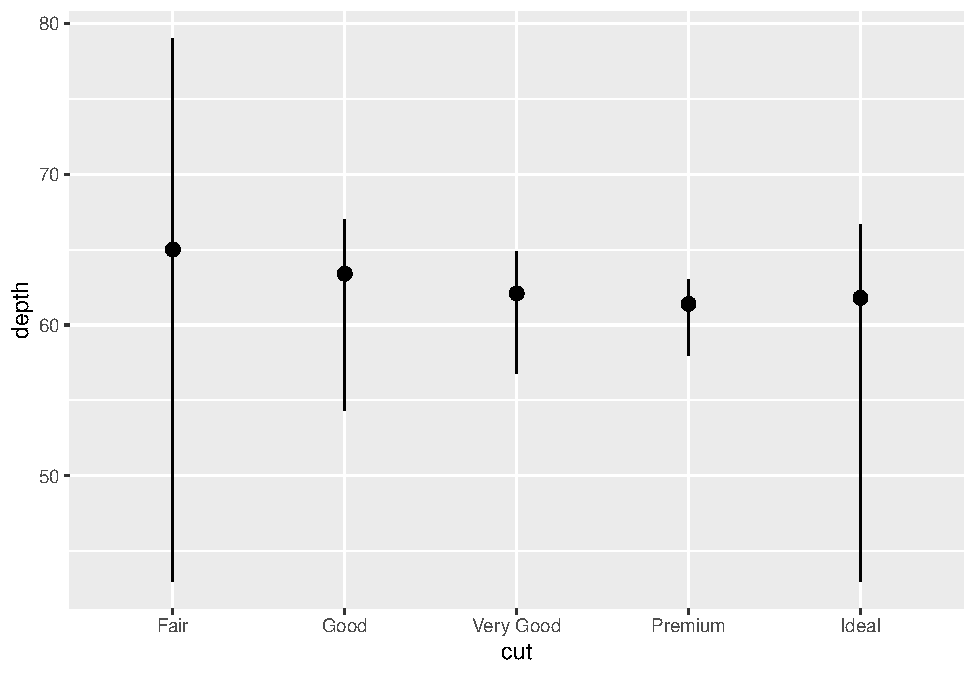
\includegraphics{r4dsexercises_files/figure-latex/3.7.1 Question 1-1.pdf}

\begin{Shaded}
\begin{Highlighting}[]
\KeywordTok{ggplot}\NormalTok{(}\DataTypeTok{data =}\NormalTok{ diamonds) }\OperatorTok{+}\StringTok{ }
\StringTok{   }\KeywordTok{geom_pointrange}\NormalTok{(}
    \DataTypeTok{mapping =} \KeywordTok{aes}\NormalTok{(}\DataTypeTok{x =}\NormalTok{ cut, }\DataTypeTok{y =}\NormalTok{ depth),}
    \DataTypeTok{stat =} \StringTok{"summary"}
\NormalTok{  )}
\end{Highlighting}
\end{Shaded}

\begin{verbatim}
## No summary function supplied, defaulting to `mean_se()`
\end{verbatim}

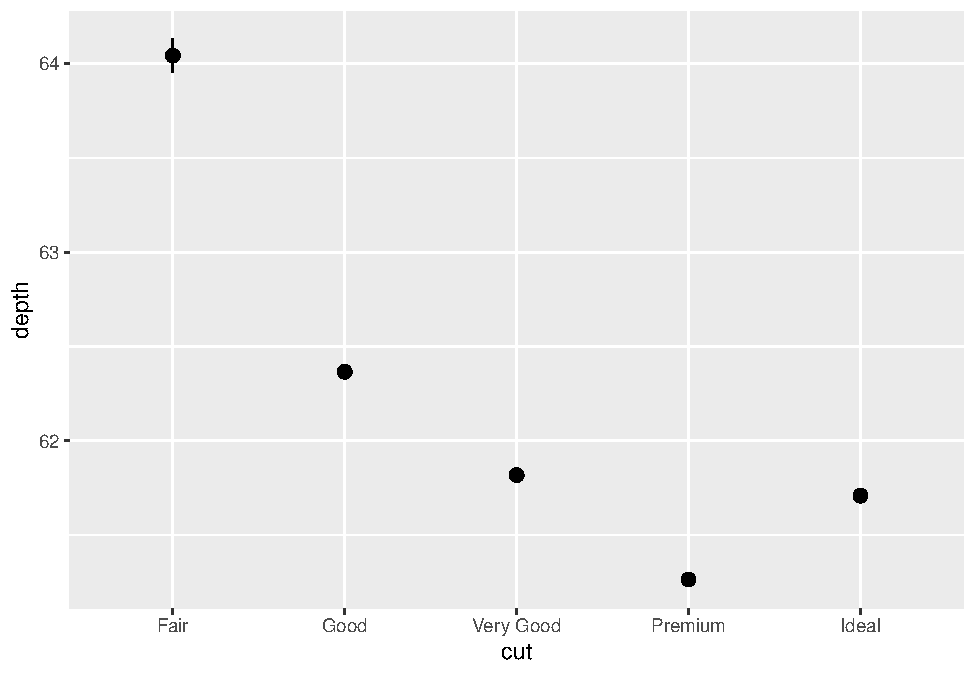
\includegraphics{r4dsexercises_files/figure-latex/3.7.1 Question 1-2.pdf}

\hypertarget{question-2-what-does-geom_col-do-how-is-it-different-to-geom_bar}{%
\subsection{Question 2: What does geom\_col() do? How is it different to geom\_bar()?}\label{question-2-what-does-geom_col-do-how-is-it-different-to-geom_bar}}

\begin{Shaded}
\begin{Highlighting}[]
\KeywordTok{ggplot}\NormalTok{(}\DataTypeTok{data =}\NormalTok{ diamonds, }\DataTypeTok{mapping =} \KeywordTok{aes}\NormalTok{(}\DataTypeTok{x =}\NormalTok{ carat, }\DataTypeTok{y =}\NormalTok{ price))}\OperatorTok{+}
\StringTok{  }\KeywordTok{geom_col}\NormalTok{()}
\end{Highlighting}
\end{Shaded}

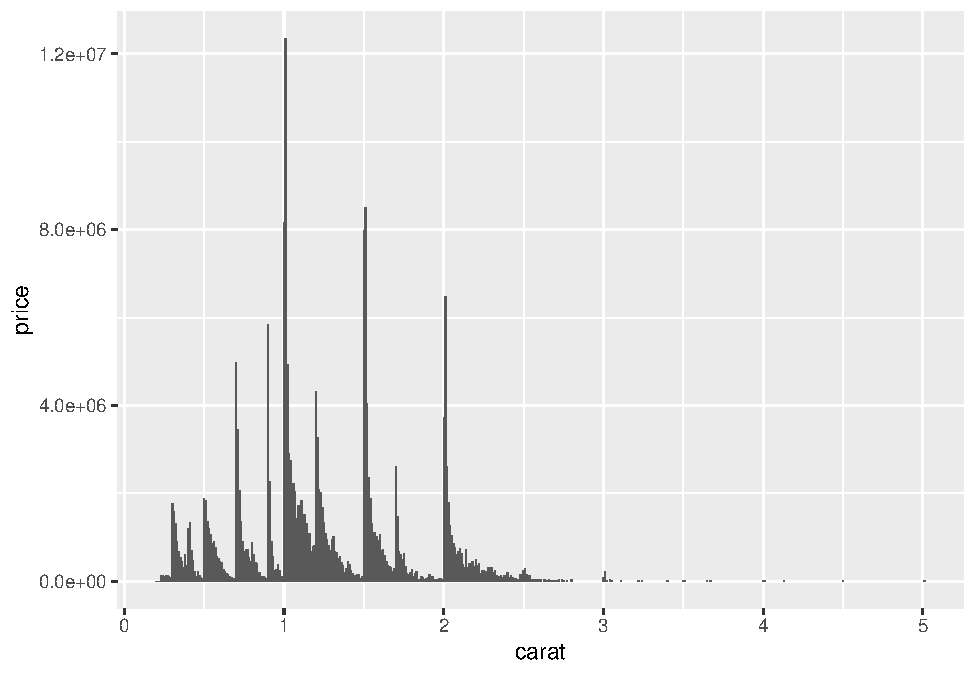
\includegraphics{r4dsexercises_files/figure-latex/3.7.1 Question 2-1.pdf}

\begin{Shaded}
\begin{Highlighting}[]
\KeywordTok{ggplot}\NormalTok{(}\DataTypeTok{data =}\NormalTok{ diamonds, }\DataTypeTok{mapping =} \KeywordTok{aes}\NormalTok{(}\DataTypeTok{x =}\NormalTok{ carat, }\DataTypeTok{y =}\NormalTok{ price))}\OperatorTok{+}
\StringTok{  }\KeywordTok{geom_bar}\NormalTok{(}\DataTypeTok{stat =} \StringTok{'identity'}\NormalTok{)}
\end{Highlighting}
\end{Shaded}

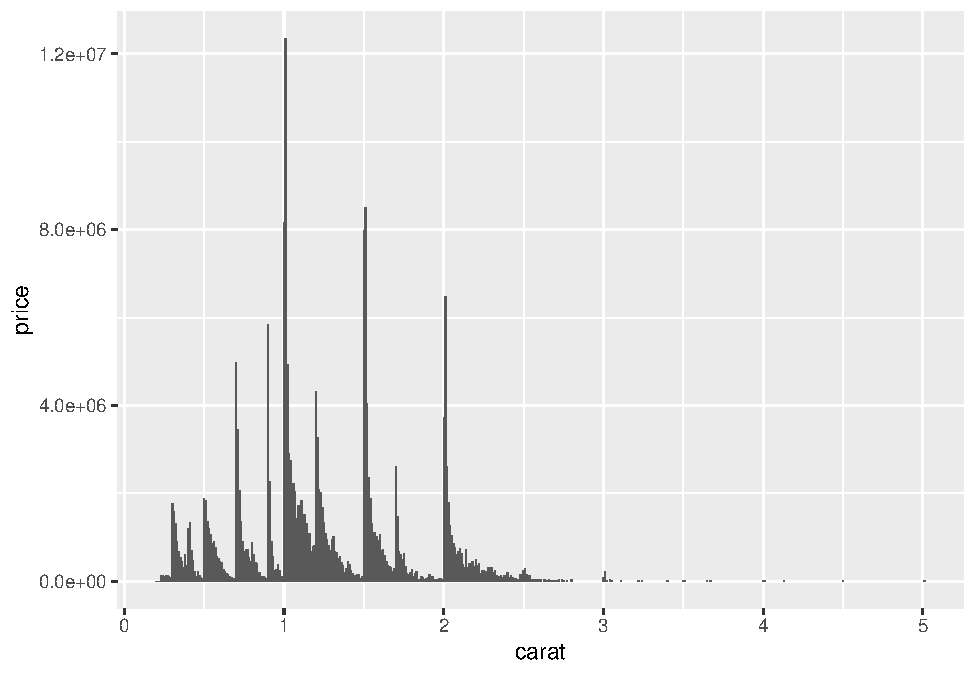
\includegraphics{r4dsexercises_files/figure-latex/3.7.1 Question 2-2.pdf}

They create the same graph but have different defaults; geom\_bar only expects an x variable wherease geom\_col requires x and y.

\hypertarget{question-3-most-geoms-and-stats-come-in-pairs-that-are-almost-always-used-in-concert.-read-through-the-documentation-and-make-a-list-of-all-the-pairs.-what-do-they-have-in-common}{%
\subsection{Question 3: Most geoms and stats come in pairs that are almost always used in concert. Read through the documentation and make a list of all the pairs. What do they have in common?}\label{question-3-most-geoms-and-stats-come-in-pairs-that-are-almost-always-used-in-concert.-read-through-the-documentation-and-make-a-list-of-all-the-pairs.-what-do-they-have-in-common}}

geom\_bar() -\textgreater{} stat\_count()
geom\_bin2d() -\textgreater{} stat\_bin\_2d()
geom\_boxplot() -\textgreater{} stat\_boxplot()
geom\_contour\_filled() -\textgreater{} stat\_contour\_filled()
geom\_contour() -\textgreater{} stat\_contour()
geom\_count() -\textgreater{} stat\_sum()
geom\_density\_2d() -\textgreater{} stat\_density\_2d()
geom\_density() -\textgreater{} stat\_density()
geom\_dotplot() -\textgreater{} stat\_bindot()
geom\_function() -\textgreater{} stat\_function()
geom\_sf() -\textgreater{} stat\_sf()
geom\_sf() -\textgreater{} stat\_sf()
geom\_smooth() -\textgreater{} stat\_smooth()
geom\_violin() -\textgreater{} stat\_ydensity()
geom\_hex() -\textgreater{} stat\_bin\_hex()
geom\_qq\_line() -\textgreater{} stat\_qq\_line()
geom\_qq() -\textgreater{} stat\_qq()
geom\_quantile() -\textgreater{} stat\_quantile()

You can see that each geom type has a stat associated with it; specific to the name and type of graph it creates.

\hypertarget{question-4-what-variables-does-stat_smooth-compute-what-parameters-control-its-behaviour}{%
\subsection{Question 4: What variables does stat\_smooth() compute? What parameters control its behaviour?}\label{question-4-what-variables-does-stat_smooth-compute-what-parameters-control-its-behaviour}}

stat\_smooth() computes: predicted values (y, x), confidence interval around the mean (ymin or xmin and ymax or ymin), and the standard error (se).

The behavior of stat\_smooth() is controlled by: na.rm, method, formula, se, method.args

\hypertarget{question-5-in-our-proportion-bar-chart-we-need-to-set-group-1.-why-in-other-words-what-is-the-problem-with-these-two-graphs}{%
\subsection{Question 5: In our proportion bar chart, we need to set group = 1. Why? In other words what is the problem with these two graphs?}\label{question-5-in-our-proportion-bar-chart-we-need-to-set-group-1.-why-in-other-words-what-is-the-problem-with-these-two-graphs}}

If group = 1 is not included, it will set the height of all the bars as the same. The issue is that the proportions are set inside the groups in this code.

\begin{Shaded}
\begin{Highlighting}[]
\KeywordTok{ggplot}\NormalTok{(}\DataTypeTok{data =}\NormalTok{ diamonds) }\OperatorTok{+}\StringTok{ }
\StringTok{  }\KeywordTok{geom_bar}\NormalTok{(}\DataTypeTok{mapping =} \KeywordTok{aes}\NormalTok{(}\DataTypeTok{x =}\NormalTok{ cut, }\DataTypeTok{y =} \KeywordTok{after_stat}\NormalTok{(prop)))}
\end{Highlighting}
\end{Shaded}

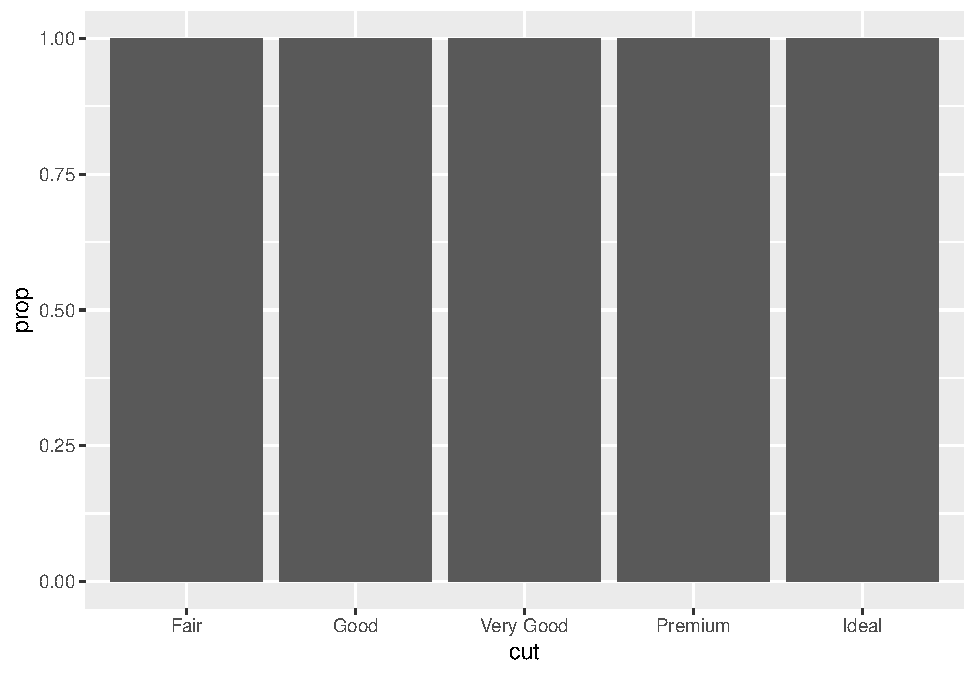
\includegraphics{r4dsexercises_files/figure-latex/3.7.1 Question 5-1.pdf}

\begin{Shaded}
\begin{Highlighting}[]
\KeywordTok{ggplot}\NormalTok{(}\DataTypeTok{data =}\NormalTok{ diamonds) }\OperatorTok{+}\StringTok{ }
\StringTok{  }\KeywordTok{geom_bar}\NormalTok{(}\DataTypeTok{mapping =} \KeywordTok{aes}\NormalTok{(}\DataTypeTok{x =}\NormalTok{ cut, }\DataTypeTok{fill =}\NormalTok{ color, }\DataTypeTok{y =} \KeywordTok{after_stat}\NormalTok{(prop)))}
\end{Highlighting}
\end{Shaded}

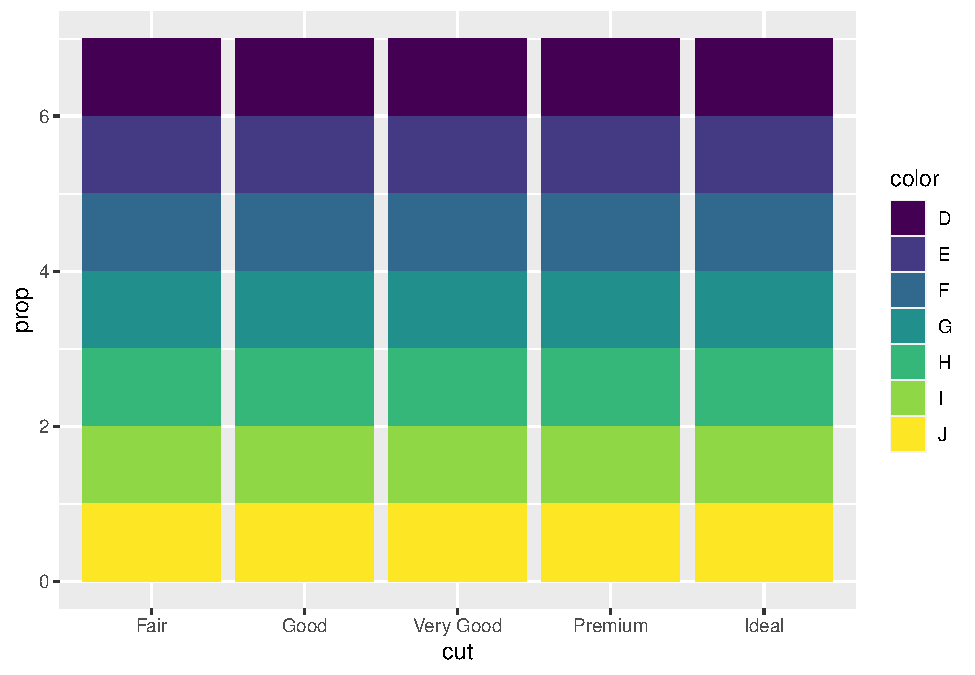
\includegraphics{r4dsexercises_files/figure-latex/3.7.1 Question 5-2.pdf}

\hypertarget{chapter-3.8.1-exercises}{%
\section{Chapter 3.8.1 Exercises}\label{chapter-3.8.1-exercises}}

\hypertarget{question-1-what-is-the-problem-with-this-plot-how-could-you-improve-it}{%
\subsection{Question 1: What is the problem with this plot? How could you improve it?}\label{question-1-what-is-the-problem-with-this-plot-how-could-you-improve-it}}

\begin{Shaded}
\begin{Highlighting}[]
\KeywordTok{ggplot}\NormalTok{(}\DataTypeTok{data =}\NormalTok{ mpg, }\DataTypeTok{mapping =} \KeywordTok{aes}\NormalTok{(}\DataTypeTok{x =}\NormalTok{ cty, }\DataTypeTok{y =}\NormalTok{ hwy)) }\OperatorTok{+}\StringTok{ }
\StringTok{  }\KeywordTok{geom_point}\NormalTok{()}
\end{Highlighting}
\end{Shaded}

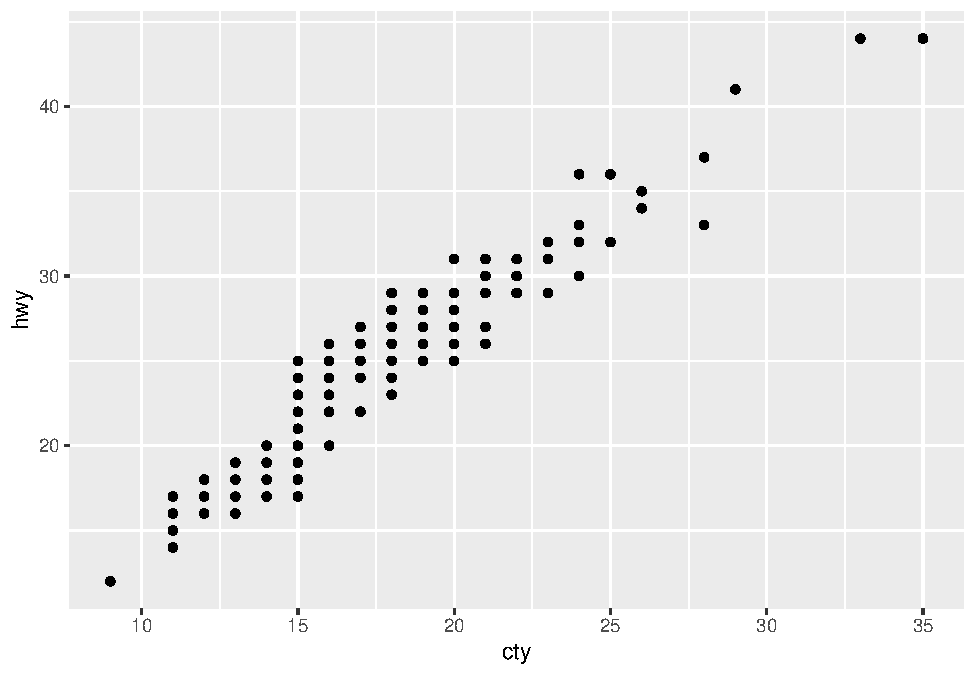
\includegraphics{r4dsexercises_files/figure-latex/3.8.1 Question 1-1.pdf}

\begin{Shaded}
\begin{Highlighting}[]
\KeywordTok{ggplot}\NormalTok{(}\DataTypeTok{data =}\NormalTok{ mpg, }\DataTypeTok{mapping =} \KeywordTok{aes}\NormalTok{(}\DataTypeTok{x =}\NormalTok{ cty, }\DataTypeTok{y =}\NormalTok{ hwy)) }\OperatorTok{+}\StringTok{ }
\StringTok{  }\KeywordTok{geom_point}\NormalTok{()}\OperatorTok{+}
\StringTok{  }\KeywordTok{geom_jitter}\NormalTok{()}
\end{Highlighting}
\end{Shaded}

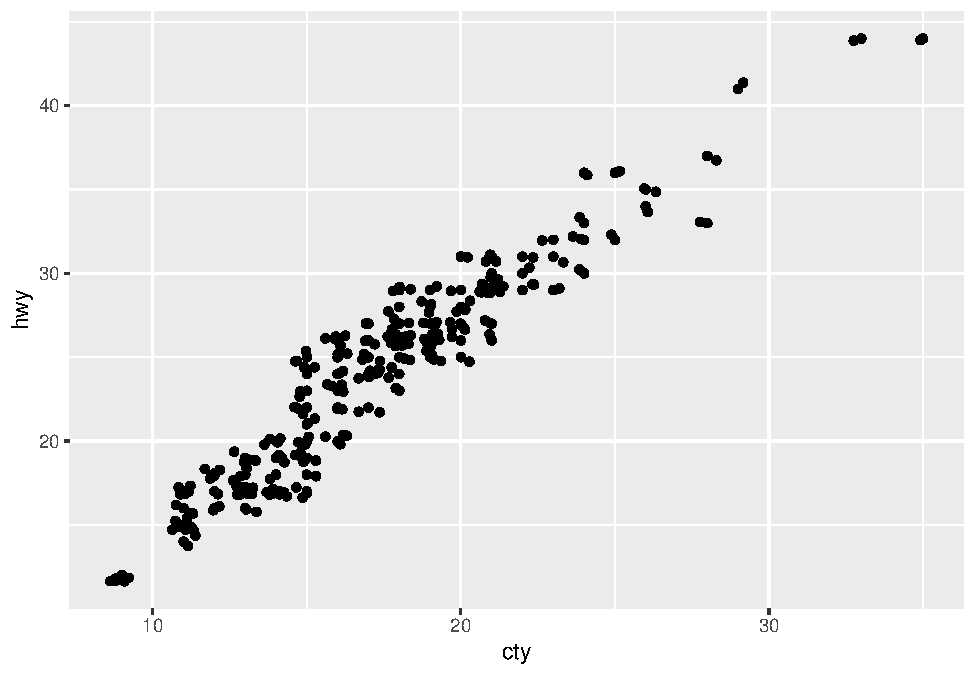
\includegraphics{r4dsexercises_files/figure-latex/3.8.1 Question 1-2.pdf}

The use of geom\_jitter() improves this plot because it makes it more visible to see the overlapping points. Without it, there is the issue of overplotting and the graph is less obvious.

\hypertarget{question-2-what-parameters-to-geom_jitter-control-the-amount-of-jittering}{%
\subsection{Question 2: What parameters to geom\_jitter() control the amount of jittering?}\label{question-2-what-parameters-to-geom_jitter-control-the-amount-of-jittering}}

width and height: the amount of vertical and horizontal jitter

\hypertarget{question-3-compare-and-contrast-geom_jitter-with-geom_count.}{%
\subsection{Question 3: Compare and contrast geom\_jitter() with geom\_count().}\label{question-3-compare-and-contrast-geom_jitter-with-geom_count.}}

geom\_jitter and geom\_count both are useful in overplotting situations as they both reveal overlapping points. Geom\_jitter makes it visible the points that overlap whereas geom\_count provides the number of points overlapping at each location on the graph.

\hypertarget{question-4-whats-the-default-position-adjustment-for-geom_boxplot-create-a-visualisation-of-the-mpg-dataset-that-demonstrates-it.}{%
\subsection{Question 4: What's the default position adjustment for geom\_boxplot()? Create a visualisation of the mpg dataset that demonstrates it.}\label{question-4-whats-the-default-position-adjustment-for-geom_boxplot-create-a-visualisation-of-the-mpg-dataset-that-demonstrates-it.}}

\begin{Shaded}
\begin{Highlighting}[]
\KeywordTok{ggplot}\NormalTok{(}\DataTypeTok{data =}\NormalTok{ mpg, }\DataTypeTok{mapping =} \KeywordTok{aes}\NormalTok{(}\DataTypeTok{x =}\NormalTok{ cty, }\DataTypeTok{y =}\NormalTok{ hwy, }\DataTypeTok{group =}\NormalTok{ drv))}\OperatorTok{+}
\StringTok{  }\KeywordTok{geom_boxplot}\NormalTok{()}
\end{Highlighting}
\end{Shaded}

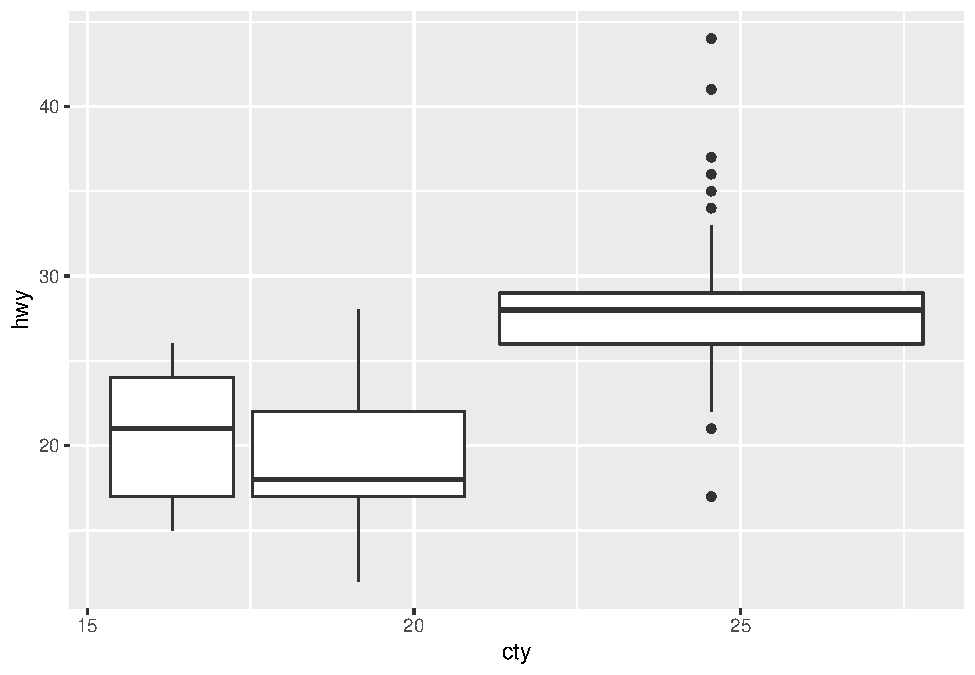
\includegraphics{r4dsexercises_files/figure-latex/3.8.1 Question 4.1-1.pdf}

The default position adjustment for geom\_boxplot() is ``dodge2.''

\begin{Shaded}
\begin{Highlighting}[]
\KeywordTok{ggplot}\NormalTok{(}\DataTypeTok{data =}\NormalTok{ mpg, }\DataTypeTok{mapping =} \KeywordTok{aes}\NormalTok{(}\DataTypeTok{x =}\NormalTok{ cty, }\DataTypeTok{y =}\NormalTok{ hwy, }\DataTypeTok{group =}\NormalTok{ drv))}\OperatorTok{+}
\StringTok{  }\KeywordTok{geom_boxplot}\NormalTok{(}\DataTypeTok{position =} \StringTok{"dodge2"}\NormalTok{)}
\end{Highlighting}
\end{Shaded}

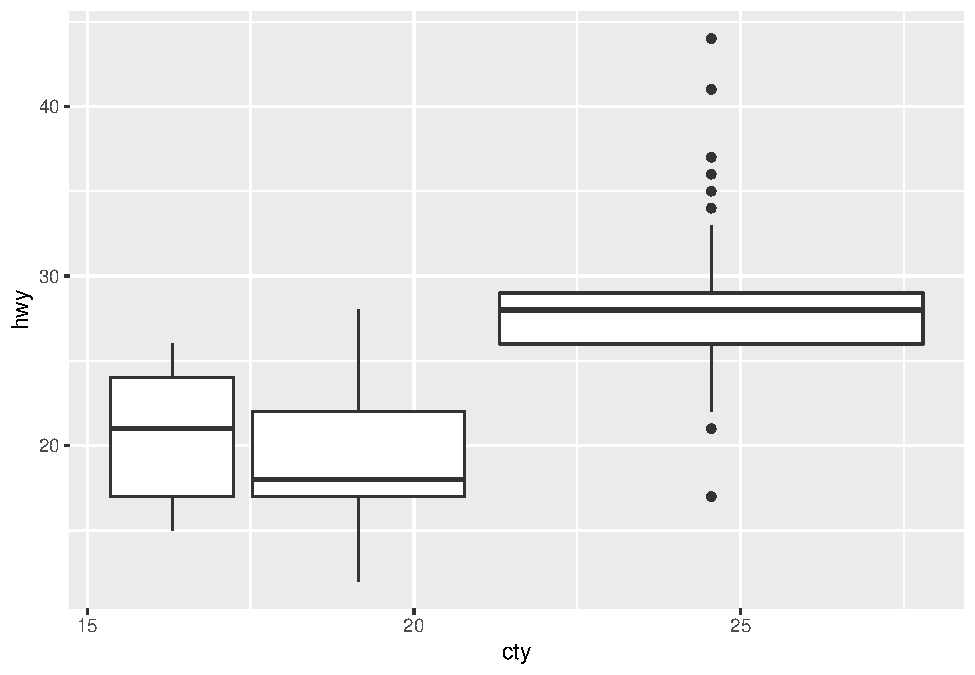
\includegraphics{r4dsexercises_files/figure-latex/3.8.1 Question 4.2-1.pdf}

Both graphs are identical, showing that the default position is `dodge2.'

\hypertarget{chapter-3.9.1-exercises}{%
\section{Chapter 3.9.1 Exercises}\label{chapter-3.9.1-exercises}}

\hypertarget{question-1-turn-a-stacked-bar-chart-into-a-pie-chart-using-coord_polar.}{%
\subsection{Question 1: Turn a stacked bar chart into a pie chart using coord\_polar().}\label{question-1-turn-a-stacked-bar-chart-into-a-pie-chart-using-coord_polar.}}

\begin{Shaded}
\begin{Highlighting}[]
\KeywordTok{ggplot}\NormalTok{(}\DataTypeTok{data =}\NormalTok{ diamonds) }\OperatorTok{+}\StringTok{ }
\StringTok{  }\KeywordTok{geom_bar}\NormalTok{(}
    \DataTypeTok{mapping =} \KeywordTok{aes}\NormalTok{(}\DataTypeTok{x =}\NormalTok{ cut, }\DataTypeTok{fill =}\NormalTok{ cut), }
    \DataTypeTok{show.legend =} \OtherTok{FALSE}\NormalTok{,}
    \DataTypeTok{width =} \DecValTok{1}
\NormalTok{  ) }\OperatorTok{+}\StringTok{ }
\StringTok{  }\KeywordTok{theme}\NormalTok{(}\DataTypeTok{aspect.ratio =} \DecValTok{1}\NormalTok{) }\OperatorTok{+}
\StringTok{  }\KeywordTok{labs}\NormalTok{(}\DataTypeTok{x =} \OtherTok{NULL}\NormalTok{, }\DataTypeTok{y =} \OtherTok{NULL}\NormalTok{)}\OperatorTok{+}
\StringTok{  }\KeywordTok{coord_flip}\NormalTok{()}
\end{Highlighting}
\end{Shaded}

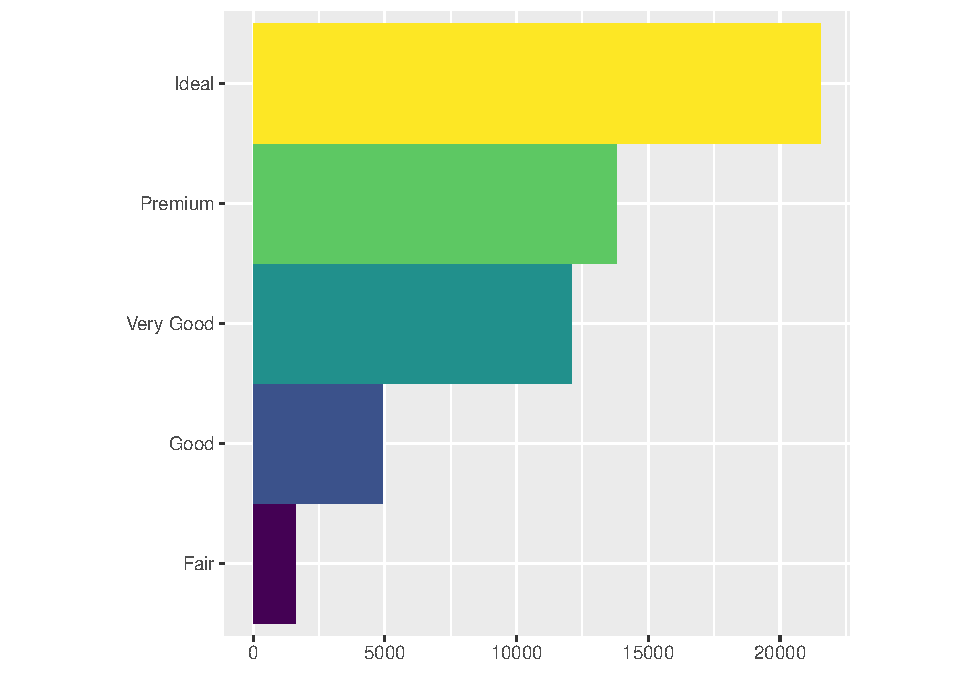
\includegraphics{r4dsexercises_files/figure-latex/3.9.1 Question 1-1.pdf}

\begin{Shaded}
\begin{Highlighting}[]
\KeywordTok{ggplot}\NormalTok{(}\DataTypeTok{data =}\NormalTok{ diamonds) }\OperatorTok{+}\StringTok{ }
\StringTok{  }\KeywordTok{geom_bar}\NormalTok{(}
    \DataTypeTok{mapping =} \KeywordTok{aes}\NormalTok{(}\DataTypeTok{x =}\NormalTok{ cut, }\DataTypeTok{fill =}\NormalTok{ cut), }
    \DataTypeTok{show.legend =} \OtherTok{FALSE}\NormalTok{,}
    \DataTypeTok{width =} \DecValTok{1}
\NormalTok{  ) }\OperatorTok{+}\StringTok{ }
\StringTok{  }\KeywordTok{theme}\NormalTok{(}\DataTypeTok{aspect.ratio =} \DecValTok{1}\NormalTok{) }\OperatorTok{+}
\StringTok{  }\KeywordTok{labs}\NormalTok{(}\DataTypeTok{x =} \OtherTok{NULL}\NormalTok{, }\DataTypeTok{y =} \OtherTok{NULL}\NormalTok{)}\OperatorTok{+}
\StringTok{  }\KeywordTok{coord_flip}\NormalTok{()}\OperatorTok{+}
\StringTok{  }\KeywordTok{coord_polar}\NormalTok{()}
\end{Highlighting}
\end{Shaded}

\begin{verbatim}
## Coordinate system already present. Adding new coordinate system, which will replace the existing one.
\end{verbatim}

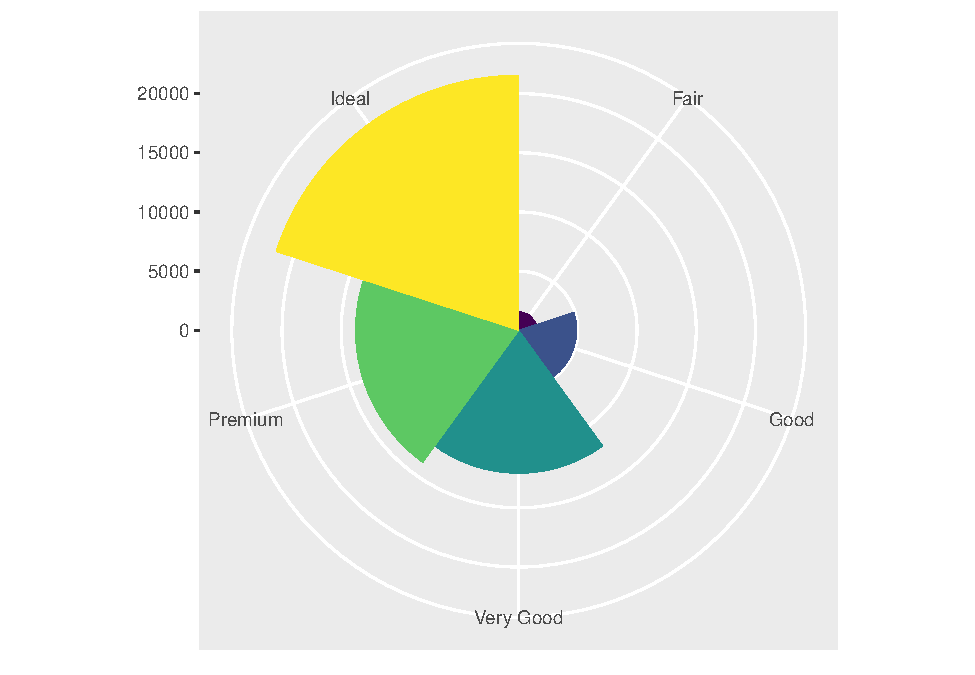
\includegraphics{r4dsexercises_files/figure-latex/3.9.1 Question 1-2.pdf}

\hypertarget{question-2-what-does-labs-do-read-the-documentation.}{%
\subsection{Question 2: What does labs() do? Read the documentation.}\label{question-2-what-does-labs-do-read-the-documentation.}}

labs() adds labels to your graph. It provides options to set a title, subtitle, caption, tag, or x/y labels.

\hypertarget{question-3-whats-the-difference-between-coord_quickmap-and-coord_map}{%
\subsection{Question 3: What's the difference between coord\_quickmap() and coord\_map()?}\label{question-3-whats-the-difference-between-coord_quickmap-and-coord_map}}

coord\_quickmap() is a quick approximation that preserves straight lines for the 2D plane from the spherical earth (so is better for smaller areas close to equator); coord\_map(), on the other hand, requires a lot of computation because it projects a portion of the earth onto a 2D plane but doesn't preserve straight lines.

\hypertarget{question-4-what-does-the-plot-below-tell-you-about-the-relationship-between-city-and-highway-mpg-why-is-coord_fixed-important-what-does-geom_abline-do}{%
\subsection{Question 4: What does the plot below tell you about the relationship between city and highway mpg? Why is coord\_fixed() important? What does geom\_abline() do?}\label{question-4-what-does-the-plot-below-tell-you-about-the-relationship-between-city-and-highway-mpg-why-is-coord_fixed-important-what-does-geom_abline-do}}

\begin{Shaded}
\begin{Highlighting}[]
\KeywordTok{ggplot}\NormalTok{(}\DataTypeTok{data =}\NormalTok{ mpg, }\DataTypeTok{mapping =} \KeywordTok{aes}\NormalTok{(}\DataTypeTok{x =}\NormalTok{ cty, }\DataTypeTok{y =}\NormalTok{ hwy)) }\OperatorTok{+}
\StringTok{  }\KeywordTok{geom_point}\NormalTok{() }\OperatorTok{+}\StringTok{ }
\StringTok{  }\KeywordTok{geom_abline}\NormalTok{() }\OperatorTok{+}
\StringTok{  }\KeywordTok{coord_fixed}\NormalTok{()}
\end{Highlighting}
\end{Shaded}

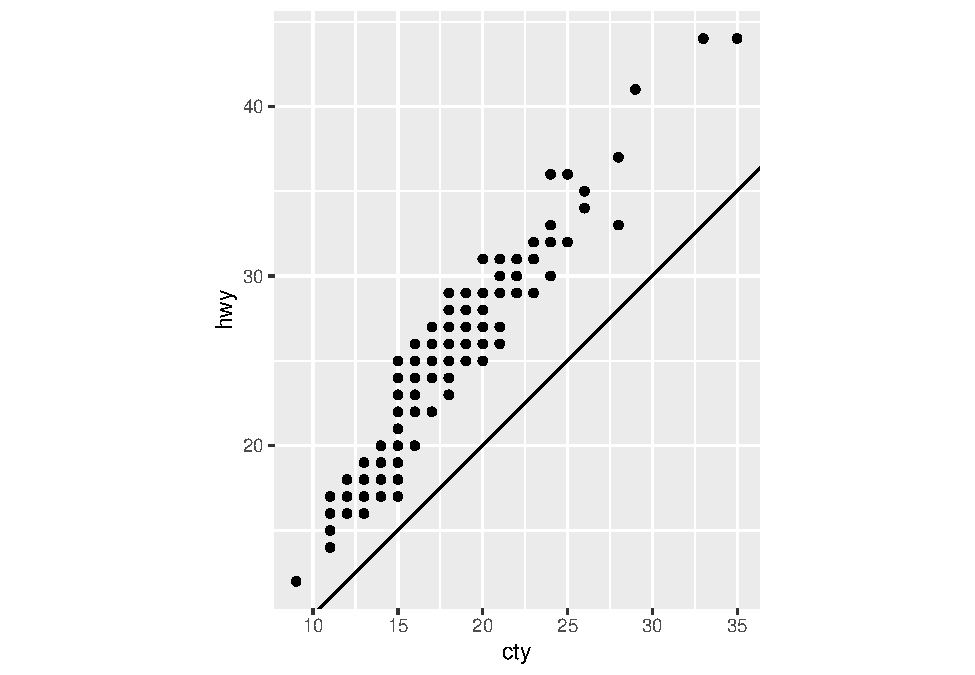
\includegraphics{r4dsexercises_files/figure-latex/3.9.1 Question 4-1.pdf}

The plot tells you that there is higher highway miles per gallon compared to city miles per gallon for all cars.
coord\_fixed() is important because it does not stretch out the graph so that it is a perfect square. It better shows the actual numerical value's position for hwy/cty.
geom\_abline() adds a reference line for the correlation between hwy and cty.

\hypertarget{chapter-4}{%
\chapter{Chapter 4}\label{chapter-4}}

\hypertarget{chapter-4.4-exercises}{%
\section{Chapter 4.4 Exercises}\label{chapter-4.4-exercises}}

\hypertarget{question-1-why-does-this-code-not-work}{%
\subsection{Question 1: Why does this code not work?}\label{question-1-why-does-this-code-not-work}}

\begin{Shaded}
\begin{Highlighting}[]
\NormalTok{my_variable <-}\StringTok{ }\DecValTok{10}
\NormalTok{my_varıable}
\end{Highlighting}
\end{Shaded}

\begin{verbatim}
## Error in eval(expr, envir, enclos): object 'my_varıable' not found
\end{verbatim}

\begin{Shaded}
\begin{Highlighting}[]
\CommentTok{#> Error in eval(expr, envir, enclos): object 'my_varıable' not found}
\end{Highlighting}
\end{Shaded}

The error is that the `i' in my\_variable is a 1 when it is attempted to be called.R needs you to be explicit with no typos when attempting to execute code.

\hypertarget{question-2-tweak-each-of-the-following-r-commands-so-that-they-run-correctly}{%
\subsection{Question 2: Tweak each of the following R commands so that they run correctly:}\label{question-2-tweak-each-of-the-following-r-commands-so-that-they-run-correctly}}

\begin{Shaded}
\begin{Highlighting}[]
\KeywordTok{ggplot}\NormalTok{(}\DataTypeTok{dota =}\NormalTok{ mpg) }\OperatorTok{+}\StringTok{ }
\StringTok{  }\KeywordTok{geom_point}\NormalTok{(}\DataTypeTok{mapping =} \KeywordTok{aes}\NormalTok{(}\DataTypeTok{x =}\NormalTok{ displ, }\DataTypeTok{y =}\NormalTok{ hwy)) }\CommentTok{#won't run}
\end{Highlighting}
\end{Shaded}

\begin{verbatim}
## Error in FUN(X[[i]], ...): object 'displ' not found
\end{verbatim}

\begin{Shaded}
\begin{Highlighting}[]
\KeywordTok{ggplot}\NormalTok{(}\DataTypeTok{data =}\NormalTok{ mpg) }\OperatorTok{+}\StringTok{ }
\StringTok{  }\KeywordTok{geom_point}\NormalTok{(}\DataTypeTok{mapping =} \KeywordTok{aes}\NormalTok{(}\DataTypeTok{x =}\NormalTok{ displ, }\DataTypeTok{y =}\NormalTok{ hwy))}
\end{Highlighting}
\end{Shaded}

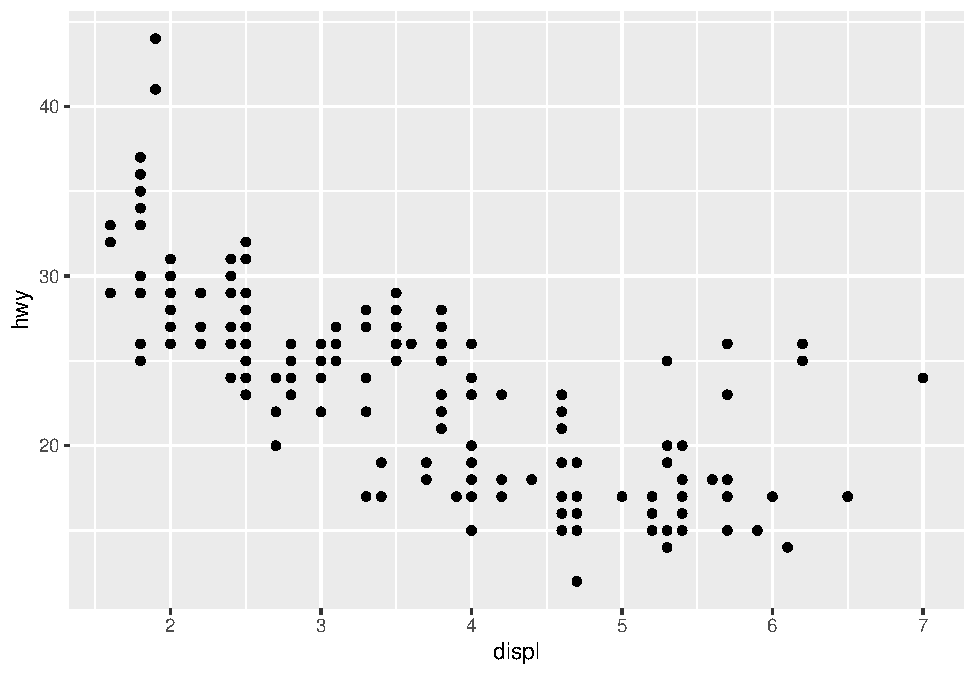
\includegraphics{r4dsexercises_files/figure-latex/4.4 Question 2-1.pdf}

\begin{Shaded}
\begin{Highlighting}[]
\KeywordTok{fliter}\NormalTok{(mpg, }\DataTypeTok{cyl =} \DecValTok{8}\NormalTok{) }\CommentTok{#won't run}
\end{Highlighting}
\end{Shaded}

\begin{verbatim}
## Error in fliter(mpg, cyl = 8): could not find function "fliter"
\end{verbatim}

\begin{Shaded}
\begin{Highlighting}[]
\KeywordTok{filter}\NormalTok{(mpg, cyl }\OperatorTok{==}\StringTok{ }\DecValTok{8}\NormalTok{)}
\end{Highlighting}
\end{Shaded}

\begin{verbatim}
## # A tibble: 70 x 11
##    manufacturer model              displ  year   cyl trans      drv     cty   hwy fl    class  
##    <chr>        <chr>              <dbl> <int> <int> <chr>      <chr> <int> <int> <chr> <chr>  
##  1 audi         a6 quattro           4.2  2008     8 auto(s6)   4        16    23 p     midsize
##  2 chevrolet    c1500 suburban 2wd   5.3  2008     8 auto(l4)   r        14    20 r     suv    
##  3 chevrolet    c1500 suburban 2wd   5.3  2008     8 auto(l4)   r        11    15 e     suv    
##  4 chevrolet    c1500 suburban 2wd   5.3  2008     8 auto(l4)   r        14    20 r     suv    
##  5 chevrolet    c1500 suburban 2wd   5.7  1999     8 auto(l4)   r        13    17 r     suv    
##  6 chevrolet    c1500 suburban 2wd   6    2008     8 auto(l4)   r        12    17 r     suv    
##  7 chevrolet    corvette             5.7  1999     8 manual(m6) r        16    26 p     2seater
##  8 chevrolet    corvette             5.7  1999     8 auto(l4)   r        15    23 p     2seater
##  9 chevrolet    corvette             6.2  2008     8 manual(m6) r        16    26 p     2seater
## 10 chevrolet    corvette             6.2  2008     8 auto(s6)   r        15    25 p     2seater
## # ... with 60 more rows
\end{verbatim}

\begin{Shaded}
\begin{Highlighting}[]
\KeywordTok{filter}\NormalTok{(diamond, carat }\OperatorTok{>}\StringTok{ }\DecValTok{3}\NormalTok{)}\CommentTok{#won't run}
\end{Highlighting}
\end{Shaded}

\begin{verbatim}
## Error in filter(diamond, carat > 3): object 'diamond' not found
\end{verbatim}

\begin{Shaded}
\begin{Highlighting}[]
\KeywordTok{filter}\NormalTok{(diamonds, carat }\OperatorTok{>}\StringTok{ }\DecValTok{3}\NormalTok{)}
\end{Highlighting}
\end{Shaded}

\begin{verbatim}
## # A tibble: 32 x 10
##    carat cut     color clarity depth table price     x     y     z
##    <dbl> <ord>   <ord> <ord>   <dbl> <dbl> <int> <dbl> <dbl> <dbl>
##  1  3.01 Premium I     I1       62.7    58  8040  9.1   8.97  5.67
##  2  3.11 Fair    J     I1       65.9    57  9823  9.15  9.02  5.98
##  3  3.01 Premium F     I1       62.2    56  9925  9.24  9.13  5.73
##  4  3.05 Premium E     I1       60.9    58 10453  9.26  9.25  5.66
##  5  3.02 Fair    I     I1       65.2    56 10577  9.11  9.02  5.91
##  6  3.01 Fair    H     I1       56.1    62 10761  9.54  9.38  5.31
##  7  3.65 Fair    H     I1       67.1    53 11668  9.53  9.48  6.38
##  8  3.24 Premium H     I1       62.1    58 12300  9.44  9.4   5.85
##  9  3.22 Ideal   I     I1       62.6    55 12545  9.49  9.42  5.92
## 10  3.5  Ideal   H     I1       62.8    57 12587  9.65  9.59  6.03
## # ... with 22 more rows
\end{verbatim}

\hypertarget{chapter-5}{%
\chapter{Chapter 5}\label{chapter-5}}

\hypertarget{chapter-5.2.4-exercises}{%
\section{Chapter 5.2.4 Exercises}\label{chapter-5.2.4-exercises}}

\hypertarget{question-1-find-all-flights-that}{%
\subsection{Question 1: Find all flights that:}\label{question-1-find-all-flights-that}}

1.1 Had an arrival delay of two or more hours

\begin{Shaded}
\begin{Highlighting}[]
\NormalTok{delay_more_}\DecValTok{2}\NormalTok{ <-}\StringTok{ }\KeywordTok{filter}\NormalTok{(nycflights13}\OperatorTok{::}\NormalTok{flights, arr_delay }\OperatorTok{>}\StringTok{ }\DecValTok{120}\NormalTok{)}
\end{Highlighting}
\end{Shaded}

10034 flights had an arrival delay of 2 or more hours

1.2 Flew to Houston (IAH or HOU)

\begin{Shaded}
\begin{Highlighting}[]
\NormalTok{flew_to_houston <-}\StringTok{ }\KeywordTok{filter}\NormalTok{(nycflights13}\OperatorTok{::}\NormalTok{flights, dest }\OperatorTok{==}\StringTok{ "IAH"} \OperatorTok{|}\StringTok{ }\NormalTok{dest }\OperatorTok{==}\StringTok{ "HOU"}\NormalTok{)}
\end{Highlighting}
\end{Shaded}

9313 flights flew to a Houston airport

1.3 Were operated by United, American, or Delta

\begin{Shaded}
\begin{Highlighting}[]
\NormalTok{un_am_del <-}\StringTok{ }\KeywordTok{filter}\NormalTok{(nycflights13}\OperatorTok{::}\NormalTok{flights, carrier }\OperatorTok{==}\StringTok{ "AA"} \OperatorTok{|}\StringTok{ }\NormalTok{carrier }\OperatorTok{==}\StringTok{ "DL"} \OperatorTok{|}\StringTok{ }\NormalTok{carrier }\OperatorTok{==}\StringTok{ "UA"}\NormalTok{)}
\end{Highlighting}
\end{Shaded}

139504 flights were operated by United, American, or Delta

1.4 Departed in summer (July, August, and September)

\begin{Shaded}
\begin{Highlighting}[]
\NormalTok{summer_flight <-}\StringTok{ }\KeywordTok{filter}\NormalTok{(nycflights13}\OperatorTok{::}\NormalTok{flights, month }\OperatorTok\StringTok{ }\KeywordTok{c}\NormalTok{(}\DecValTok{7}\NormalTok{,}\DecValTok{8}\NormalTok{,}\DecValTok{9}\NormalTok{))}
\end{Highlighting}
\end{Shaded}

86326 flights departed in summer

1.5 Arrived more than two hours late, but didn't leave late

\begin{Shaded}
\begin{Highlighting}[]
\NormalTok{arr_}\DecValTok{2}\NormalTok{_late_dep_on_time <-}\StringTok{ }\KeywordTok{filter}\NormalTok{(nycflights13}\OperatorTok{::}\NormalTok{flights, dep_delay }\OperatorTok{<=}\StringTok{ }\DecValTok{0} \OperatorTok{&}\StringTok{ }\NormalTok{arr_delay }\OperatorTok{>}\StringTok{ }\DecValTok{120}\NormalTok{)}
\end{Highlighting}
\end{Shaded}

29 flights arrived more than 2 hours late, but left on time or early.

1.6 Were delayed by at least an hour, but made up over 30 minutes in flight

\begin{Shaded}
\begin{Highlighting}[]
\NormalTok{made_up_}\DecValTok{30}\NormalTok{ <-}\StringTok{ }\KeywordTok{filter}\NormalTok{(nycflights13}\OperatorTok{::}\NormalTok{flights, dep_delay }\OperatorTok{>=}\StringTok{ }\DecValTok{60} \OperatorTok{&}\StringTok{ }\NormalTok{((dep_delay }\OperatorTok{-}\StringTok{ }\NormalTok{arr_delay) }\OperatorTok{>}\StringTok{ }\DecValTok{30}\NormalTok{))}
\end{Highlighting}
\end{Shaded}

1844 flights were delayed by at least an hour but made up over 30 minutes in air

1.7 Departed between midnight and 6am (inclusive)

\begin{Shaded}
\begin{Highlighting}[]
\NormalTok{overnight_flight_dep <-}\StringTok{ }\KeywordTok{filter}\NormalTok{(nycflights13}\OperatorTok{::}\NormalTok{flights, dep_time }\OperatorTok\StringTok{ }\KeywordTok{c}\NormalTok{(}\DecValTok{12}\NormalTok{,}\DecValTok{1}\NormalTok{,}\DecValTok{2}\NormalTok{,}\DecValTok{3}\NormalTok{,}\DecValTok{4}\NormalTok{,}\DecValTok{5}\NormalTok{,}\DecValTok{6}\NormalTok{))}
\end{Highlighting}
\end{Shaded}

177 flights left between midnight and 6am

\hypertarget{question-2-another-useful-dplyr-filtering-helper-is-between.-what-does-it-do-can-you-use-it-to-simplify-the-code-needed-to-answer-the-previous-challenges}{%
\subsection{Question 2: Another useful dplyr filtering helper is between(). What does it do? Can you use it to simplify the code needed to answer the previous challenges?}\label{question-2-another-useful-dplyr-filtering-helper-is-between.-what-does-it-do-can-you-use-it-to-simplify-the-code-needed-to-answer-the-previous-challenges}}

between() will select the rows of values that fall within a specific range. Must be a numeric vector.You could simplify the last exercise (1.7) by:

\begin{Shaded}
\begin{Highlighting}[]
\NormalTok{overnight_dep <-}\StringTok{ }\KeywordTok{filter}\NormalTok{(nycflights13}\OperatorTok{::}\NormalTok{flights, }\KeywordTok{between}\NormalTok{(dep_time, }\DecValTok{1}\NormalTok{, }\DecValTok{6}\NormalTok{) }\OperatorTok{|}\StringTok{ }\NormalTok{dep_time }\OperatorTok{==}\DecValTok{12}\NormalTok{)}
\end{Highlighting}
\end{Shaded}

\hypertarget{question-3-how-many-flights-have-a-missing-dep_time-what-other-variables-are-missing-what-might-these-rows-represent}{%
\subsection{Question 3: How many flights have a missing dep\_time? What other variables are missing? What might these rows represent?}\label{question-3-how-many-flights-have-a-missing-dep_time-what-other-variables-are-missing-what-might-these-rows-represent}}

\begin{Shaded}
\begin{Highlighting}[]
\NormalTok{missing_dep_time <-}\StringTok{ }\KeywordTok{filter}\NormalTok{(nycflights13}\OperatorTok{::}\NormalTok{flights, }\KeywordTok{is.na}\NormalTok{(dep_time))}
\end{Highlighting}
\end{Shaded}

8255 flights have a missing departure time

These flights are also missing a dep\_delay and arr\_time, so these may represent the flights that were cancelled.

\hypertarget{question-4-why-is-na-0-not-missing-why-is-na-true-not-missing-why-is-false-na-not-missing-can-you-figure-out-the-general-rule-na-0-is-a-tricky-counterexample}{%
\subsection{Question 4: Why is NA \^{} 0 not missing? Why is NA \textbar{} TRUE not missing? Why is FALSE \& NA not missing? Can you figure out the general rule? (NA * 0 is a tricky counterexample!)}\label{question-4-why-is-na-0-not-missing-why-is-na-true-not-missing-why-is-false-na-not-missing-can-you-figure-out-the-general-rule-na-0-is-a-tricky-counterexample}}

NA \^{} 0 = 1 because everything to the 0th power is 1.
NA \textbar{} TRUE it'll still return the the result of the boolean.
FALSE \& NA will return the result of the boolean.
The general rule is that it will return the boolean value.
NA*0 = NA because when you try to do math on an NA value, it will return NA

\hypertarget{chapter-5.3.1-exercises}{%
\section{Chapter 5.3.1 Exercises}\label{chapter-5.3.1-exercises}}

\hypertarget{question-1-how-could-you-use-arrange-to-sort-all-missing-values-to-the-start-hint-use-is.na.}{%
\subsection{Question 1: How could you use arrange() to sort all missing values to the start? (Hint: use is.na()).}\label{question-1-how-could-you-use-arrange-to-sort-all-missing-values-to-the-start-hint-use-is.na.}}

\begin{Shaded}
\begin{Highlighting}[]
\KeywordTok{arrange}\NormalTok{(flights, }\KeywordTok{desc}\NormalTok{(}\KeywordTok{is.na}\NormalTok{(flights)))}
\end{Highlighting}
\end{Shaded}

\begin{verbatim}
## # A tibble: 336,776 x 22
##     year month   day dep_time sched_dep_time dep_delay arr_time sched_arr_time arr_delay carrier flight tailnum origin
##    <int> <int> <int>    <int>          <int>     <dbl>    <int>          <int>     <dbl> <chr>    <int> <chr>   <chr> 
##  1  2013     1     2       NA           1545        NA       NA           1910        NA AA         133 <NA>    JFK   
##  2  2013     1     2       NA           1601        NA       NA           1735        NA UA         623 <NA>    EWR   
##  3  2013     1     3       NA            857        NA       NA           1209        NA UA         714 <NA>    EWR   
##  4  2013     1     3       NA            645        NA       NA            952        NA UA         719 <NA>    EWR   
##  5  2013     1     4       NA            845        NA       NA           1015        NA 9E        3405 <NA>    JFK   
##  6  2013     1     4       NA           1830        NA       NA           2044        NA 9E        3716 <NA>    EWR   
##  7  2013     1     5       NA            840        NA       NA           1001        NA 9E        3422 <NA>    JFK   
##  8  2013     1     7       NA            820        NA       NA            958        NA 9E        3317 <NA>    JFK   
##  9  2013     1     8       NA           1645        NA       NA           1838        NA US         123 <NA>    EWR   
## 10  2013     1     9       NA            755        NA       NA           1012        NA 9E        4023 <NA>    EWR   
## # ... with 336,766 more rows, and 9 more variables: dest <chr>, air_time <dbl>, distance <dbl>, hour <dbl>, minute <dbl>,
## #   time_hour <dttm>, speed <dbl>, min_since_mid_dep_time <dbl>, min_since_mid_sched_dep_time <dbl>
\end{verbatim}

\hypertarget{question-2-sort-flights-to-find-the-most-delayed-flights.-find-the-flights-that-left-earliest.}{%
\subsection{Question 2: Sort flights to find the most delayed flights. Find the flights that left earliest.}\label{question-2-sort-flights-to-find-the-most-delayed-flights.-find-the-flights-that-left-earliest.}}

\begin{Shaded}
\begin{Highlighting}[]
\NormalTok{most_delay <-}\StringTok{ }\KeywordTok{arrange}\NormalTok{(flights, }\KeywordTok{desc}\NormalTok{(dep_delay))}

\NormalTok{most_delay }\OperatorTok\StringTok{ }
\StringTok{  }\KeywordTok{arrange}\NormalTok{(dep_time)}
\end{Highlighting}
\end{Shaded}

\begin{verbatim}
## # A tibble: 336,776 x 22
##     year month   day dep_time sched_dep_time dep_delay arr_time sched_arr_time arr_delay carrier flight tailnum origin
##    <int> <int> <int>    <int>          <int>     <dbl>    <int>          <int>     <dbl> <chr>    <int> <chr>   <chr> 
##  1  2013     4    10        1           1930       271      106           2101       245 UA        1703 N33203  EWR   
##  2  2013     5    22        1           1935       266      154           2140       254 EV        4361 N27200  EWR   
##  3  2013     6    24        1           1950       251      105           2130       215 AA         363 N546AA  LGA   
##  4  2013     7     1        1           2029       212      236           2359       157 B6         915 N653JB  JFK   
##  5  2013     1    31        1           2100       181      124           2225       179 WN         530 N550WN  LGA   
##  6  2013     2    11        1           2100       181      111           2225       166 WN         530 N231WN  LGA   
##  7  2013     3    18        1           2128       153      247           2355       172 B6          97 N760JB  JFK   
##  8  2013     6    25        1           2130       151      249             14       155 B6        1371 N607JB  LGA   
##  9  2013     2    24        1           2245        76      121           2354        87 B6         608 N216JB  JFK   
## 10  2013     1    13        1           2249        72      108           2357        71 B6          22 N206JB  JFK   
## # ... with 336,766 more rows, and 9 more variables: dest <chr>, air_time <dbl>, distance <dbl>, hour <dbl>, minute <dbl>,
## #   time_hour <dttm>, speed <dbl>, min_since_mid_dep_time <dbl>, min_since_mid_sched_dep_time <dbl>
\end{verbatim}

\hypertarget{question-3-sort-flights-to-find-the-fastest-highest-speed-flights.}{%
\subsection{Question 3: Sort flights to find the fastest (highest speed) flights.}\label{question-3-sort-flights-to-find-the-fastest-highest-speed-flights.}}

\begin{Shaded}
\begin{Highlighting}[]
\NormalTok{flights <-}\StringTok{ }\NormalTok{flights }\OperatorTok\StringTok{ }
\StringTok{  }\KeywordTok{mutate}\NormalTok{(}\DataTypeTok{speed =}\NormalTok{ distance}\OperatorTok{/}\NormalTok{hour)}

\NormalTok{fastest_flights <-}\StringTok{ }\KeywordTok{arrange}\NormalTok{(flights, }\KeywordTok{desc}\NormalTok{(speed))}
\end{Highlighting}
\end{Shaded}

\hypertarget{question-4-which-flights-travelled-the-farthest-which-travelled-the-shortest}{%
\subsection{Question 4: Which flights travelled the farthest? Which travelled the shortest?}\label{question-4-which-flights-travelled-the-farthest-which-travelled-the-shortest}}

\begin{Shaded}
\begin{Highlighting}[]
\NormalTok{far <-}\StringTok{ }\KeywordTok{arrange}\NormalTok{(flights, }\KeywordTok{desc}\NormalTok{(distance))}

\NormalTok{short <-}\StringTok{ }\KeywordTok{arrange}\NormalTok{(flights, distance)}
\end{Highlighting}
\end{Shaded}

\hypertarget{chapter-5.4.1-exercises}{%
\section{Chapter 5.4.1 Exercises}\label{chapter-5.4.1-exercises}}

\hypertarget{question-1-brainstorm-as-many-ways-as-possible-to-select-dep_time-dep_delay-arr_time-and-arr_delay-from-flights.}{%
\subsection{Question 1: Brainstorm as many ways as possible to select dep\_time, dep\_delay, arr\_time, and arr\_delay from flights.}\label{question-1-brainstorm-as-many-ways-as-possible-to-select-dep_time-dep_delay-arr_time-and-arr_delay-from-flights.}}

\begin{Shaded}
\begin{Highlighting}[]
\NormalTok{flights }\OperatorTok\StringTok{ }\KeywordTok{select}\NormalTok{(}\KeywordTok{matches}\NormalTok{(}\StringTok{"^dep_"}\NormalTok{),}\KeywordTok{matches}\NormalTok{(}\StringTok{"^arr_"}\NormalTok{))}
\end{Highlighting}
\end{Shaded}

\begin{verbatim}
## # A tibble: 336,776 x 4
##    dep_time dep_delay arr_time arr_delay
##       <int>     <dbl>    <int>     <dbl>
##  1      517         2      830        11
##  2      533         4      850        20
##  3      542         2      923        33
##  4      544        -1     1004       -18
##  5      554        -6      812       -25
##  6      554        -4      740        12
##  7      555        -5      913        19
##  8      557        -3      709       -14
##  9      557        -3      838        -8
## 10      558        -2      753         8
## # ... with 336,766 more rows
\end{verbatim}

\begin{Shaded}
\begin{Highlighting}[]
\NormalTok{flights }\OperatorTok\StringTok{ }\KeywordTok{select}\NormalTok{(dep_time, dep_delay, arr_time, arr_delay)}
\end{Highlighting}
\end{Shaded}

\begin{verbatim}
## # A tibble: 336,776 x 4
##    dep_time dep_delay arr_time arr_delay
##       <int>     <dbl>    <int>     <dbl>
##  1      517         2      830        11
##  2      533         4      850        20
##  3      542         2      923        33
##  4      544        -1     1004       -18
##  5      554        -6      812       -25
##  6      554        -4      740        12
##  7      555        -5      913        19
##  8      557        -3      709       -14
##  9      557        -3      838        -8
## 10      558        -2      753         8
## # ... with 336,766 more rows
\end{verbatim}

\begin{Shaded}
\begin{Highlighting}[]
\CommentTok{# you can also select by column position number}
\NormalTok{flights }\OperatorTok\StringTok{  }\KeywordTok{select}\NormalTok{(}\DecValTok{4}\NormalTok{,}\DecValTok{6}\NormalTok{,}\DecValTok{7}\NormalTok{,}\DecValTok{9}\NormalTok{)}
\end{Highlighting}
\end{Shaded}

\begin{verbatim}
## # A tibble: 336,776 x 4
##    dep_time dep_delay arr_time arr_delay
##       <int>     <dbl>    <int>     <dbl>
##  1      517         2      830        11
##  2      533         4      850        20
##  3      542         2      923        33
##  4      544        -1     1004       -18
##  5      554        -6      812       -25
##  6      554        -4      740        12
##  7      555        -5      913        19
##  8      557        -3      709       -14
##  9      557        -3      838        -8
## 10      558        -2      753         8
## # ... with 336,766 more rows
\end{verbatim}

*these are the reasonable ways to do this, you could do ridiculous things like subtracting every name but those you want

\hypertarget{question-2-what-happens-if-you-include-the-name-of-a-variable-multiple-times-in-a-select-call}{%
\subsection{Question 2: What happens if you include the name of a variable multiple times in a select() call?}\label{question-2-what-happens-if-you-include-the-name-of-a-variable-multiple-times-in-a-select-call}}

\begin{Shaded}
\begin{Highlighting}[]
\NormalTok{flights }\OperatorTok\StringTok{ }\KeywordTok{select}\NormalTok{(year, year, month,day, year)}
\end{Highlighting}
\end{Shaded}

\begin{verbatim}
## # A tibble: 336,776 x 3
##     year month   day
##    <int> <int> <int>
##  1  2013     1     1
##  2  2013     1     1
##  3  2013     1     1
##  4  2013     1     1
##  5  2013     1     1
##  6  2013     1     1
##  7  2013     1     1
##  8  2013     1     1
##  9  2013     1     1
## 10  2013     1     1
## # ... with 336,766 more rows
\end{verbatim}

It will only print the variable one time, regardless of how many times you call the variable name in select()

\hypertarget{question-3-what-does-the-any_of-function-do-why-might-it-be-helpful-in-conjunction-with-this-vector}{%
\subsection{Question 3: What does the any\_of() function do? Why might it be helpful in conjunction with this vector?}\label{question-3-what-does-the-any_of-function-do-why-might-it-be-helpful-in-conjunction-with-this-vector}}

\begin{Shaded}
\begin{Highlighting}[]
\NormalTok{vars <-}\StringTok{ }\KeywordTok{c}\NormalTok{(}\StringTok{"year"}\NormalTok{, }\StringTok{"month"}\NormalTok{, }\StringTok{"day"}\NormalTok{, }\StringTok{"dep_delay"}\NormalTok{, }\StringTok{"arr_delay"}\NormalTok{)}
\NormalTok{flights }\OperatorTok\StringTok{  }\KeywordTok{select}\NormalTok{(}\KeywordTok{any_of}\NormalTok{(vars))}
\end{Highlighting}
\end{Shaded}

\begin{verbatim}
## # A tibble: 336,776 x 5
##     year month   day dep_delay arr_delay
##    <int> <int> <int>     <dbl>     <dbl>
##  1  2013     1     1         2        11
##  2  2013     1     1         4        20
##  3  2013     1     1         2        33
##  4  2013     1     1        -1       -18
##  5  2013     1     1        -6       -25
##  6  2013     1     1        -4        12
##  7  2013     1     1        -5        19
##  8  2013     1     1        -3       -14
##  9  2013     1     1        -3        -8
## 10  2013     1     1        -2         8
## # ... with 336,766 more rows
\end{verbatim}

any\_of() select variables in a character vector and does not check for missing variables.

\hypertarget{question-4-does-the-result-of-running-the-following-code-surprise-you-how-do-the-select-helpers-deal-with-case-by-default-how-can-you-change-that-default}{%
\subsection{Question 4: Does the result of running the following code surprise you? How do the select helpers deal with case by default? How can you change that default?}\label{question-4-does-the-result-of-running-the-following-code-surprise-you-how-do-the-select-helpers-deal-with-case-by-default-how-can-you-change-that-default}}

\begin{Shaded}
\begin{Highlighting}[]
\KeywordTok{select}\NormalTok{(flights, }\KeywordTok{contains}\NormalTok{(}\StringTok{"TIME"}\NormalTok{))}
\end{Highlighting}
\end{Shaded}

\begin{verbatim}
## # A tibble: 336,776 x 8
##    dep_time sched_dep_time arr_time sched_arr_time air_time time_hour           min_since_mid_dep_time min_since_mid_sched~
##       <int>          <int>    <int>          <int>    <dbl> <dttm>                               <dbl>                <dbl>
##  1      517            515      830            819      227 2013-01-01 05:00:00                    317                  315
##  2      533            529      850            830      227 2013-01-01 05:00:00                    333                  329
##  3      542            540      923            850      160 2013-01-01 05:00:00                    342                  340
##  4      544            545     1004           1022      183 2013-01-01 05:00:00                    344                  345
##  5      554            600      812            837      116 2013-01-01 06:00:00                    354                  360
##  6      554            558      740            728      150 2013-01-01 05:00:00                    354                  358
##  7      555            600      913            854      158 2013-01-01 06:00:00                    355                  360
##  8      557            600      709            723       53 2013-01-01 06:00:00                    357                  360
##  9      557            600      838            846      140 2013-01-01 06:00:00                    357                  360
## 10      558            600      753            745      138 2013-01-01 06:00:00                    358                  360
## # ... with 336,766 more rows
\end{verbatim}

No, as the code prints all the variables that contain the string ``time'' within it. The default is that ignore.case = TRUE, so the capitalization within the code wouldn't effect the output. You can change ignore.case = FALSE to make it case dependent.

\hypertarget{exercises}{%
\section{5.5.2 Exercises}\label{exercises}}

\hypertarget{question-1-currently-dep_time-and-sched_dep_time-are-convenient-to-look-at-but-hard-to-compute-with-because-theyre-not-really-continuous-numbers.-convert-them-to-a-more-convenient-representation-of-number-of-minutes-since-midnight.}{%
\subsection{Question 1: Currently dep\_time and sched\_dep\_time are convenient to look at, but hard to compute with because they're not really continuous numbers. Convert them to a more convenient representation of number of minutes since midnight.}\label{question-1-currently-dep_time-and-sched_dep_time-are-convenient-to-look-at-but-hard-to-compute-with-because-theyre-not-really-continuous-numbers.-convert-them-to-a-more-convenient-representation-of-number-of-minutes-since-midnight.}}

\begin{Shaded}
\begin{Highlighting}[]
\NormalTok{flights <-}\StringTok{ }\NormalTok{flights }\OperatorTok\StringTok{ }
\StringTok{  }\KeywordTok{mutate}\NormalTok{(}\DataTypeTok{min_since_mid_dep_time =}\NormalTok{ dep_time }\OperatorTok\StringTok{ }\DecValTok{100} \OperatorTok{*}\StringTok{ }\DecValTok{60} \OperatorTok{+}\StringTok{ }\NormalTok{dep_time }\OperatorTok\StringTok{ }\DecValTok{100}\NormalTok{)}

\NormalTok{flights <-}\StringTok{ }\NormalTok{flights }\OperatorTok\StringTok{ }
\StringTok{  }\KeywordTok{mutate}\NormalTok{(}\DataTypeTok{min_since_mid_sched_dep_time =}\NormalTok{ sched_dep_time}\OperatorTok\StringTok{ }\DecValTok{100} \OperatorTok{*}\StringTok{ }\DecValTok{60} \OperatorTok{+}\StringTok{ }\NormalTok{sched_dep_time }\OperatorTok\StringTok{ }\DecValTok{100}\NormalTok{)}
\end{Highlighting}
\end{Shaded}

\hypertarget{question-2-compare-air_time-with-arr_time---dep_time.-what-do-you-expect-to-see-what-do-you-see-what-do-you-need-to-do-to-fix-it}{%
\subsection{Question 2: Compare air\_time with arr\_time - dep\_time. What do you expect to see? What do you see? What do you need to do to fix it?}\label{question-2-compare-air_time-with-arr_time---dep_time.-what-do-you-expect-to-see-what-do-you-see-what-do-you-need-to-do-to-fix-it}}

\begin{Shaded}
\begin{Highlighting}[]
\KeywordTok{head}\NormalTok{(flights}\OperatorTok{$}\NormalTok{air_time)}
\end{Highlighting}
\end{Shaded}

\begin{verbatim}
## [1] 227 227 160 183 116 150
\end{verbatim}

\begin{Shaded}
\begin{Highlighting}[]
\NormalTok{airtime2 <-}\StringTok{ }\NormalTok{flights}\OperatorTok{$}\NormalTok{arr_time }\OperatorTok{-}\StringTok{ }\NormalTok{flights}\OperatorTok{$}\NormalTok{dep_time}
\KeywordTok{head}\NormalTok{(airtime2)}
\end{Highlighting}
\end{Shaded}

\begin{verbatim}
## [1] 313 317 381 460 258 186
\end{verbatim}

The air\_time's are smaller than the (arr\_time-dep\_time)'s. This is because the arr\_time and dep\_time are written not in the minutes since midnight but rather just the hourminutes of time (i.e.~315 = 3:15) together. air\_time is the total amount of time spent in the air in minutes. Therefore, to fix this, you should use calculate the minutes

  \bibliography{book.bib,packages.bib}

\end{document}
